\documentclass[11pt,a4paper]{ctexart}
\usepackage[margin=2.3cm]{geometry}
\usepackage{graphicx,booktabs,amsmath,amssymb,array,caption,float,xcolor,hyperref,microtype,needspace}
\hypersetup{colorlinks=true,linkcolor=blue!50!black,citecolor=blue!50!black,urlcolor=blue!50!black}
\captionsetup{font=small,labelfont=bf}
\setlength{\parskip}{4pt}\setlength{\parindent}{0pt}
\title{SOAD：融合跨视图聚合与质量校准的观测感知柑橘检测}
\author{作者信息待补}
\date{}
\begin{document}
\maketitle

\begin{abstract}
密集柑橘检测是机器人自主采摘的重要感知环节，果实尺度小、相邻实例遮挡和背景外观相似使准确定位与误检控制面临困难。本文提出\textbf{采样算子感知检测器（Sampling-Operator-Aware Detector，SOAD）}，将输入观测保留、跨块实例聚合与候选质量估计结合为完整检测流程。该方法以原生像素重叠图块组织训练和推理，使果实的局部轮廓与外观细节进入 RT-DETR-L 检测网络，并通过边界筛选、坐标还原和整图去重形成实例预测。进一步利用镜像视图的互补预测融合目标位置，结合候选证据分别估计检测正确性与定位质量，得到校准后的检测得分。校准器在验证集上单独学习，检测器权重保持固定。在跨果园留出集和相近训练迭代预算下，完整 SOAD 相对整图 RT-DETR-L 基线的 mAP50:95 提高了 33.3\%，在召回率为 0.70 时每图误检数降低了 77.2\%。该方法提高了密集小果实的检出能力和高召回率下的背景排除能力，为果园果实定位、数量估计与机器人采摘目标筛选提供视觉感知支持。
\end{abstract}
\textbf{关键词：} 柑橘检测；小目标；原始分辨率切块；RGB-D；置信度校准；果实计数

\section{引言}
面向机器人采摘的柑橘检测与计数 \cite{agyolo,mfaf,geosphere}，旨在从野外图像中定位每个果实并估计其数量，是农业机器人视觉感知中的基础问题。这一问题本质上是不适定的，因为叶片遮挡、果实重叠和相似颜色背景会使不同的果实边界或实例排列产生近似的二维观测；仅凭单幅图像，解并不总是唯一。现有方法通常利用颜色、上下文、形状或深度几何等先验缩小可能的解空间。与实验室图像分析不同，自动采摘还要求感知结果及时送达机器人控制系统，而野外部署的相机分辨率、边缘设备算力和能耗均受约束，不能依赖无限提高采集与推理分辨率。因而，小果实在输入图像中只有有限的像素支持，是检测与计数必须面对的基本条件。

GeoSphere-DETR \cite{geosphere} 是利用几何先验处理柑橘检测的代表性方法之一。该方法将 RGB 图像和深度数据调整至网络输入尺度，分别提取多尺度视觉特征和曲率线索，通过几何门控预测候选框，再依据几何一致性调整得分并完成计数。RT-DETR 系列 \cite{rtdetr,rtdetrv2} 重点优化特征编码和查询选择，AG-YOLO \cite{agyolo}、MFAF-YOLO \cite{mfaf} 等方法则增强果园场景中的特征与跨尺度融合。这些改进作用于输入采样之后，其效果仍受果实在网络输入中保留的可辨识细节约束。SAHI \cite{sahi} 和 ASAHI \cite{asahi} 已证明切片有利于小目标检测，但在果园 RGB-D 场景中，切片保留的视觉信息会改变几何线索能够补充的信息量。当相邻果实的边界或果实与黄叶的差异被压缩到少数像素时，几何融合带来的框排序改善与得分变化需要分别检验。

输入缩放改变果实轮廓、相邻实例间隔和背景差异在网络中的可辨识程度。被采样抹去的差异无法由后续 RGB 特征编码唯一恢复，因此输入组织直接影响检测器能够学习的实例表征。深度几何提供额外观测，其增益取决于 RGB 输入保留的信息以及几何数据的对齐质量。本文利用原生像素图块组织训练和推理，通过跨块归属与整图聚合生成实例预测，并在相同输入条件下评估几何融合与决策校准。

我们将所提出的流程称为\textbf{采样算子感知检测器}（Sampling-Operator-Aware Detector，\textbf{SOAD}）。SOAD 从传感图像生成保留原有像素尺度的重叠图块，并依据目标与图块的交叠面积分配训练标注，使训练与推理中的目标具有一致的输入尺度。检测器分别预测各图块中的果实，随后剔除靠近图块内部边界的截断框，将其余候选框映射至整图坐标并去重。原图与镜像图的预测在统一坐标系中融合，以减小定位波动；检测正确性和框定位质量的校准结果用于调整候选框得分。完整流程在跨果园留出集上的 mAP50:95 较整图基线相对提高了 33.3\%。

\Needspace{10\baselineskip}
总体而言，本文的贡献主要有以下三个方面。
\begin{enumerate}
\item 建立\emph{观测算子--目标表征--几何增益}的条件化分析框架。把传感图像、确定性采样和检测决策表示为连续的信息链，用统计最优风险的信息顺序刻画输入采样的不可逆约束，并以目标在特征层的有效空间支持连接局部判别、框定位与实例分离；在同一框架下，将深度的潜在收益定义为给定 RGB 采样结果后的条件风险差，而非将多模态融合预设为必然有效。
\item 构建采样算子感知的柑橘实例检测流程 SOAD。以原生像素重叠图块组织检测输入，在训练阶段通过目标面积归属生成图块标注并控制空块比例，在推理阶段结合内边界筛选、坐标回映射与整图去重保持跨图块实例一致；随后融合镜像视图的候选框，降低局部预测的定位波动。
\item 构造检测正确性与定位质量的分解式校准损失。对候选框分别建立果实匹配标签和匹配后的 IoU 目标，以二元对数损失训练真果概率估计，以平方损失训练质量回归，再按验证集选择的权重组合两项预测得分。该损失作用于检测后的校准模型，使得分同时反映实例真实性与框定位质量，并通过特征消融检验深度、曲率等证据的实际作用。
\end{enumerate}

输入采样决定后续表征可利用的视觉证据，也影响深度几何的条件增益。以下依次讨论相关方法、SOAD 的实现与实验结果，并讨论各环节的性能贡献与计算代价。

\section{相关工作}
\subsection{实时检测与果园柑橘检测}
实时目标检测研究主要通过特征编码、查询匹配和边界框回归协调精度与计算开销。RT-DETR \cite{rtdetr} 利用高效混合编码器和考虑 IoU 的查询选择实现端到端检测，RT-DETRv2 \cite{rtdetrv2} 进一步优化多尺度采样与训练策略。2025 年的 D-FINE \cite{dfine} 将边界框回归表示为逐层细化的概率分布，并通过定位自蒸馏改善回归质量；DEIM \cite{deim} 则通过增加每幅训练图像中的目标数量强化一对一匹配监督，利用匹配感知损失改善不同质量样本的优化。这些工作分别提高了表征效率、定位精度和监督利用率，但网络内部的优化仍以输入中已经保留的目标信息为前提，无法直接补偿整图缩放在特征提取之前消除的实例差异。针对这一输入约束，\textbf{SOAD} 将原生像素图块作为训练与推理的共同观测单位，并通过整图实例聚合将局部判别结果还原为完整检测输出。

果园检测器进一步将通用网络适配到枝叶遮挡、光照变化与果实尺度差异。AG-YOLO \cite{agyolo} 和 MFAF-YOLO \cite{mfaf} 分别利用全局上下文与多尺度自适应融合增强果实特征。2025 年的 YOLO-MECD \cite{mecd} 面向树上果实与落果检测，将高效多尺度注意力、部分卷积模块和 MPDIoU 损失结合，在减少模型规模的同时改善检测性能。2026 年的 ACDNet \cite{acdnet} 采用果实感知特征提取、动态多尺度采样和形状感知 IoU 损失，使采样位置及定位监督适应柑橘形态。上述方法已关注小果实与遮挡问题，但其特征采样和形状约束仍作用于网络接收到的观测，输入压缩造成的轮廓与实例间隔损失并不会因增加注意力或形状先验而自动消除。\textbf{SOAD} 因此在特征学习之前保留局部像素尺度，并通过目标面积归属和内边界筛选处理切块产生的截断实例，将输入细节与实例完整性共同纳入检测流程。

近期研究也开始直接处理特征降采样引起的细节退化。SCORE-DETR（2025）\cite{scoredetr} 针对小尺寸和遮挡柑橘构建频率聚合网络与 Haar 小波融合模块，以增强目标信号并缓解多尺度融合中的混叠。FG-DETR（2026）\cite{fgdetr} 进一步组合动态特征编码、空间与频率域增强以及小波降采样，在抑制复杂背景响应的同时保留高频细节。这一方向说明细节保护已成为果园检测的重要研究内容，其所保护的是网络内部已有的特征信息，进入网络之前被缩放移除的目标差异仍处于该机制的作用范围之外。\textbf{SOAD} 将细节保护前移到观测组织阶段，以原生像素图块减少额外输入压缩，并用观测算子与检测风险的关系说明这一设计对后续特征学习的意义。

\subsection{小目标切片与跨视图实例聚合}
切片检测通过将大幅图像分解为局部输入，提高小目标在固定网络尺寸下的有效空间占比。SAHI \cite{sahi} 将重叠切片推理与切片辅助微调结合，已经同时考虑局部输入及训练适配。2026 年的 ASAHI 预印本 \cite{asahi} 根据图像分辨率调整切片数量，结合整图与切片训练样本，并采用 Cluster-DIoU-NMS 处理重复检测，重点改善固定切片尺寸带来的冗余计算。切片与去重能够改善目标可见尺度，但密集果实在重叠区域同时呈现同一实例的重复观测和不同实例的相互交叠，仅以框间几何相似性聚合仍面临截断框归属与相邻实例区分的问题。\textbf{SOAD} 在训练时按目标交叠面积分配标注，在推理时先筛除内部切块边界附近的截断候选，再执行坐标回映射和整图去重，使实例归属规则贯穿局部学习与全图输出。

跨视图融合进一步利用同一实例的多个预测缓解定位波动。加权框融合 \cite{wbf} 按置信度聚合同类候选框的坐标，提供了利用多预测定位信息的通用方式；ASAHI \cite{asahi} 则通过中心距离与重叠关系组织重复框抑制。二者分别侧重候选框坐标整合与重复检测消除，在密集检测中都需要以可靠的实例匹配为基础。上述几何聚合本身不等价于候选真实性建模，相似背景产生的错误框也可能具有较高得分或跨视图一致性。\textbf{SOAD} 因此将镜像框融合与证据校准分开设计，先在统一坐标系中整合定位信息，再利用候选上下文及框相关证据调整最终得分。

\subsection{RGB-D 融合与几何信息的条件增益}
RGB-D 果实检测利用颜色纹理与空间结构的互补关系缓解外观歧义。GeoSphere-DETR（2026）\cite{geosphere} 从深度中构建曲率线索，通过可学习空间门控选择几何特征，并在候选层引入几何一致性重评分。该方法已经显式处理深度可靠性和相似背景误检，几何信息因而同时参与表征学习与输出决策。然而，几何可靠性建模并不直接回答新增观测相对于既有 RGB 证据的条件贡献，RGB 输入压缩程度变化时，同一几何线索所补充的判别信息也会变化。\textbf{SOAD} 将输入采样纳入检测风险分析，并以同步裁剪和同步增强的 RGB--几何图块建立独立对照，考察保留局部视觉证据后几何信息的附加作用。

几何表征的来源也决定了融合结果应如何解释。CIAFNet（2026）\cite{ciafnet} 采用跨模态交互、自适应融合和多尺度聚合，在自然果园中使用由 Depth Anything V2 生成的伪深度，并在受控场景中进一步适配传感器实测深度。伪深度从同一 RGB 图像推断结构先验，实测深度则来自额外传感观测，二者在信息来源、缺失模式与噪声分布上存在区别。上述融合机制解决了结构表征的选择与适配问题，但将结构表征带来的学习便利直接解释为独立传感信息增益，仍会混淆表征先验、观测质量和输入尺度的作用。\textbf{SOAD} 据此区分 RGB 观测组织与附加几何证据，在保持图块尺度和空间对应关系一致的条件下分析几何收益，使模态贡献与检测输入条件相联系。

\subsection{检测正确性与定位质量校准}
检测置信度需要同时支持候选排序与阈值筛选，而类别得分不必然与边界框定位质量一致。Bridging Precision and Confidence \cite{bpc} 在检测器训练阶段引入校准损失，以缩小置信度与检测正确性之间的差距。Lee 等于 2026 年在线发表的工作 \cite{trackcal} 则利用视频跟踪框提供时间一致的定位参照，并以 IoU 感知加权损失减弱跟踪噪声对无标注后校准的影响。上述方法分别依赖检测训练阶段的校准约束或视频中的时间参照，无法直接替代独立果园图像经跨块与镜像聚合后所需的候选质量估计。\textbf{SOAD} 在冻结检测器后，以验证集候选框的匹配正确性和匹配 IoU 分别监督分类与质量回归，形成适用于整图聚合输出的分解式校准目标。

针对果实误检，GeoSphere-DETR \cite{geosphere} 的几何重评分将形状一致性转化为候选筛选依据；跟踪辅助校准 \cite{trackcal} 则从时间一致性构造质量参照。这些方法表明，得分调整的关键在于辅助证据是否与真实检测质量一致，而非单纯改变分数范围。单一几何或时间一致性证据仍受深度缺失、局部遮挡及对应关系误差制约，不能完整描述独立静态图像中候选真实性与定位质量的差别。\textbf{SOAD} 将检测得分、图内上下文和框相关描述纳入候选证据，通过正确性与定位质量的分解学习形成重评分，并在特征移除对照和固定召回率误检分析中检验各类证据的实际贡献。

\section{方法}
\subsection{整体框架}
SOAD 从 RGB 图像生成原生像素图块，在相同尺度的图块上训练和推理，并将局部检测还原为整图实例。镜像融合与证据重新评分作用于检测输出。为了测量几何线索的条件收益，另以 GeoSphere-DETR 建立同步输入 RGB 与 B／N 曲率图的独立对照。图~\ref{fig:pipe} 展示各操作在训练和推理中的位置。

\begin{figure}[H]
\centering
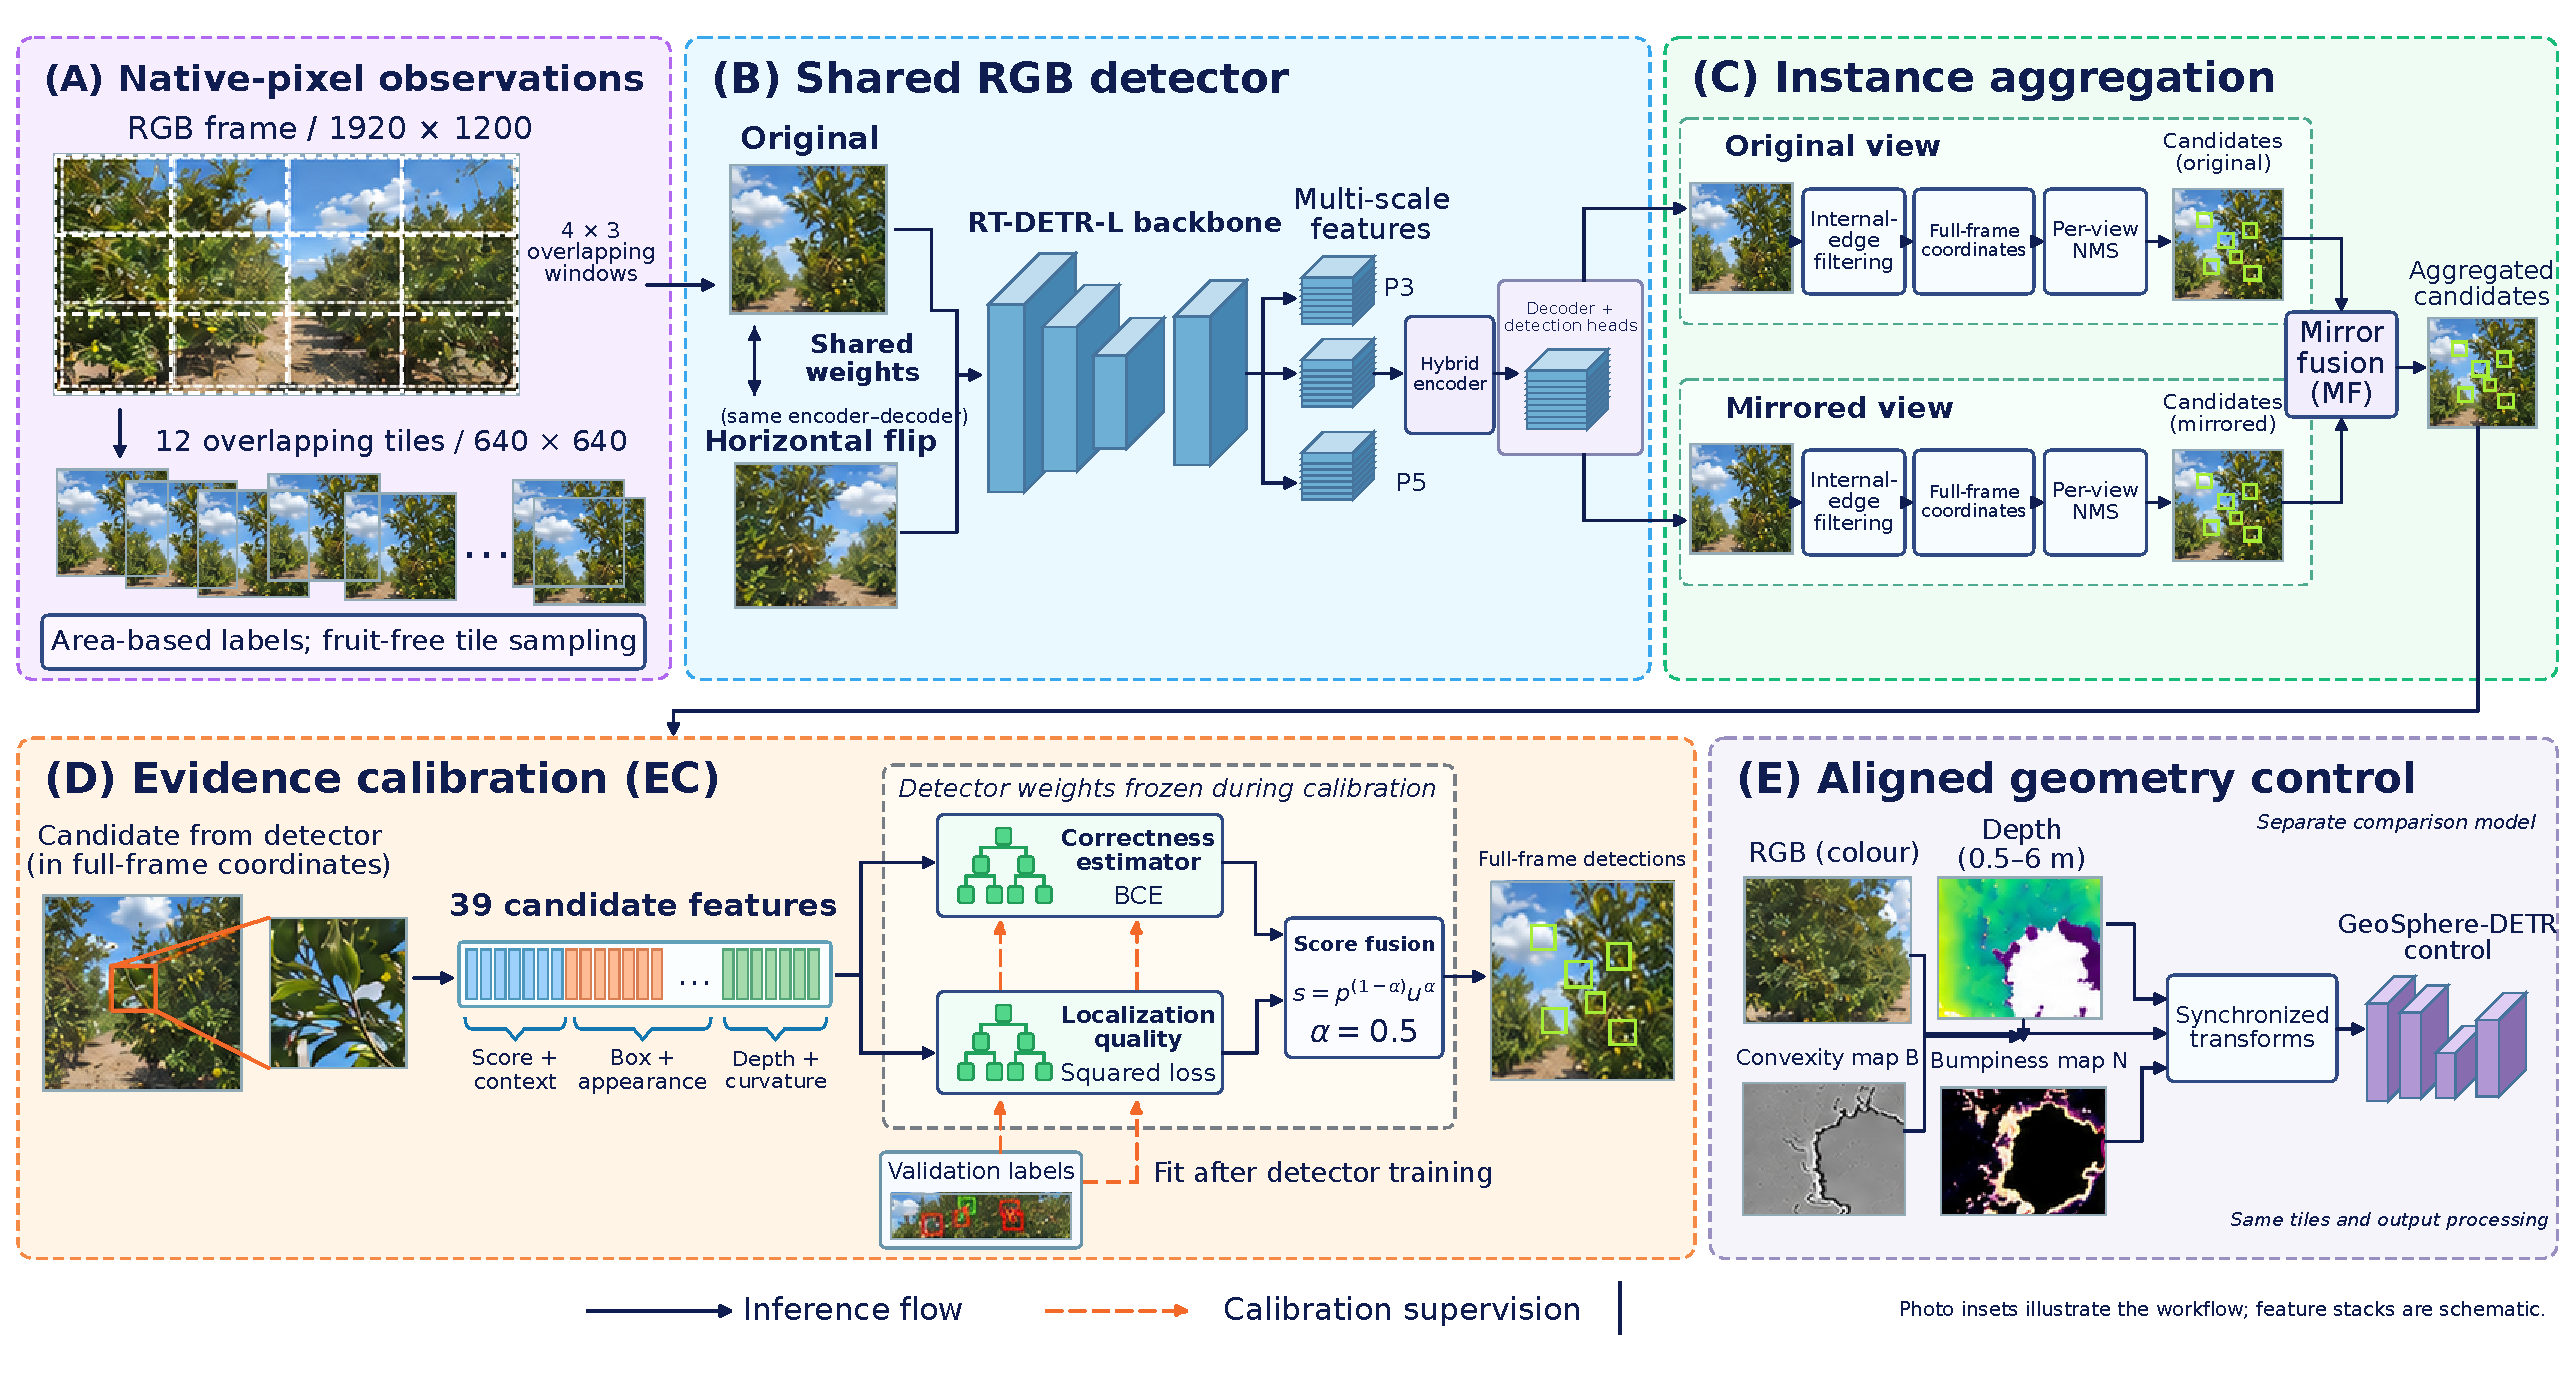
\includegraphics[width=0.98\linewidth]{../figures/fig_pipeline.pdf}
\caption{\textbf{SOAD} 的整体框架。（A）原生像素重叠图块与训练标注组织；（B）原始视图和镜像视图共用 RT-DETR-L 检测网络；（C）逐视图边界筛选、坐标还原及去重，随后进行镜像融合（MF）；（D）利用候选证据分别估计检测正确性与定位质量，融合得到校准得分（EC）。校准器由验证集监督单独拟合，检测器权重固定。（E）同步 RGB 与 B／N 曲率图的独立几何对照，不属于主检测网络。}
\label{fig:pipe}
\end{figure}
图~\ref{fig:pipe} 将 SOAD 的设计分为局部观测保留、实例坐标恢复和候选质量调整三个环节。重叠图块提供原生像素尺度的局部输入，坐标回映射与整图去重将局部预测转化为可计数的实例集合，镜像融合与证据校准进一步处理定位和筛选。该结构把输入组织与实例输出连接为完整检测流程，明确了各项方法设计之间的依赖关系，并为后续模块消融提供结构依据。

\subsection{观测算子与检测风险}
\label{sec:observation}
令 $I\in\mathbb{R}^{H\times W\times3}$ 为传感器 RGB 图像，$Y$ 为果实类别与边界框构成的标注集合，$G\in\mathbb{R}^{H\times W\times2}$ 为可选的深度派生几何图。给定检测或计数损失 $\ell$，对任意观测 $Z$ 定义不限制模型容量时的最优统计风险
\begin{equation}
\mathcal{R}^{*}(Z)=\inf_{f}\mathbb{E}\!\left[\ell\bigl(f(Z),Y\bigr)\right].
\end{equation}
设 $D_S$ 为将整图缩至网络宽度 $S$ 的确定性算子。每个基于 $D_S(I)$ 的决策都可由一个先计算 $D_S$、再执行同一决策的完整图像模型模拟，因此
\begin{equation}
\mathcal{R}^{*}(I)\leq\mathcal{R}^{*}\!\bigl(D_S(I)\bigr).
\label{eq:risk}
\end{equation}
式~\eqref{eq:risk} 在不限制判别函数容量的条件下刻画完整观测与缩放观测之间的信息顺序，为保留相机已采集的局部细节提供理论依据。有限容量检测器的实际收益由训练与评估检验。加入几何观测后的理论条件收益为 $\Delta_G^{*}(D_S)=\mathcal{R}^{*}(D_S(I))-\mathcal{R}^{*}(D_S(I),G)\geq0$，其大小依赖输入算子和 $G$ 的信息质量。本文据此在相同图块和同步对齐条件下测量几何模型的性能增量，将理论上的信息增量与实际模型表现联系起来。

检测器的特征层还把输入算子的作用转化为空间支持。若果实在传感图像中的宽度为 $w$，输入变换的缩放因子为 $\alpha$，特征层步长为 $q_\ell$，则该层上的近似目标跨度为 $\rho_\ell=\alpha w/q_\ell$。这并非检测成功的阈值，但说明相同网络中的目标表征、框定位与相邻实例分离会随采样算子改变。本文数据的图像宽为 1920 像素，整图输入宽度为 640 像素时 $\alpha\approx1/3$；果实框边长中位数为 21.1 像素，对应输入跨度约为 7.0 像素。这是本数据上的量级说明，式~\eqref{eq:risk} 与 $\rho_\ell$ 的关系不依赖这些特定数值。

\subsection{原生像素图块训练}

将每幅 1920$\times$1200 图像划为 $4\times3$ 个 640$\times$640 图块，横向起点为 $\{0,427,853,1280\}$，纵向起点为 $\{0,280,560\}$。相邻图块重叠 213 或 280 像素。一个标注框与图块交集面积达到自身面积的至少一半时，才分配给该图块并裁剪至图块边界。训练保留全部含果实图块，并以固定随机种子保留四分之一无果实图块；验证和测试使用每幅图像的全部十二个图块。14,792 个训练图块来自 1,492 幅可加载训练图像，包含 184,642 个图块级框。批量大小为 8，训练十轮约 18,490 次迭代，接近整图训练一百轮的 18,700 次。模型仍为 COCO 预训练的 RT-DETR-L，损失函数和骨干保持不变。

\subsection{图块推理、边界处理与整图去重}
设图块原点为 $(x_t,y_t)$，图块坐标框 $b_t=(x_1,y_1,x_2,y_2)$ 通过加上原点映回整图。若检测框接触内部图块边界的距离不超过 2 像素，则舍弃该框；重叠区域使相邻图块仍能观察到完整果实。保留框按类别使用 IoU 阈值 0.5 的非极大值抑制去重，最后仅保留得分最高的 300 个框，与单次整图检测的输出上限一致。边界规则是确定性的，避免对截断果实的坐标进行不稳定平均。

\subsection{镜像融合与可选的得分校准}
对每个图块再执行一次水平镜像推理，将镜像检测映回原坐标。参考加权框融合 \cite{wbf}，相同类别的框以 IoU 0.55 贪心聚类；对簇 $\mathcal{C}$，坐标采用置信度加权均值
\begin{equation}
\bar b=\frac{\sum_{j\in\mathcal{C}}s_j b_j}{\sum_{j\in\mathcal{C}}s_j},
\qquad
\bar s=\frac{\sum_{j\in\mathcal{C}}s_j}{2}.
\end{equation}
第二式按两个视图归一，因此仅由一个视图发现的框得分较低。此步骤需要 24 次而非 12 次网络推理。

对置信度高于 0.02 的检测，校准器计算得分及图内上下文、框形状、深度及周围环带、物理尺寸、曲率图与 HSV 颜色，共 39 项候选特征。设候选框 $i$ 在 IoU 0.5 下的果实匹配标签为 $y_i\in\{0,1\}$，与同类别标注的最大重叠率为 $q_i$。分类模型 $p_\theta(x_i)$ 估计真果概率，回归模型 $u_\phi(x_i)$ 估计质量目标 $y_iq_i$。两个梯度提升模型 \cite{lgbm} 分别最小化二元对数损失和平方损失；由于参数独立，其训练可写为分解式校准目标
\begin{equation}
\mathcal{L}_{\mathrm{cal}}=\sum_i\ell_{\mathrm{BCE}}\!\left(y_i,p_\theta(x_i)\right)
+\sum_i\left(u_\phi(x_i)-y_iq_i\right)^2.
\label{eq:cal_loss}
\end{equation}
校准得分将两项预测按指数权重组合，具体为
\begin{equation}
s_{\mathrm{cal}}=\hat p^{1-\alpha}\hat u^{\alpha},\qquad \alpha=0.5.
\end{equation}
模型和 $\alpha$ 仅通过验证集按图像分组的五折折外预测选择；留出果园从不用于拟合。式~\eqref{eq:cal_loss} 描述检测后的校准训练，RT-DETR-L 骨干未使用这一损失。深度和曲率特征的贡献通过移除对应特征后的性能差值评价。

\subsection{对齐几何输入的控制比较}
为了判断几何线索在尺度得到保护后是否仍有收益，将 B、N 曲率图作为 RGB 之外的第四、第五通道，并使马赛克、仿射和翻转同时作用于五个通道；颜色扰动只作用于 RGB。增强结束后再分离几何图，输入参考架构的门控分支。这样比较的 RGB 与几何模型拥有相同图块、训练轮次、推理和评价协议。几何门控分支在此作为受控比较对象，不属于主要 RGB 流程。

\section{实验与结果}
\subsection{数据、划分与评价协议}
我们使用公开的 RGB-D 柑橘数据集 \cite{dataset,geosphere}，包含 2,200 幅图像和 102,719 个标注实例，按 1,500／200／500 幅划分训练、验证和测试。测试图像来自不同果园和采集日期。每幅图像包含 1920$\times$1200 RGB 帧、毫米单位的 16 位深度图、B／N 曲率图，以及树上和地面果实标注。本节依次检验数据与观测条件、图块输入的检测收益、校准目标的作用，以及几何输入的条件收益与计算代价。所有性能结论均在整图坐标系下计算。

\begin{table}[H]
\centering
\small
\caption{RGB-D 柑橘数据集的划分与类别分布。}
\label{tab:data}
\begin{tabular}{lrrrr}
\toprule
数据划分 & 图像数 & 树上果实 & 地面果实 & 实例总数 \\
\midrule
训练集 & 1,500 & 71,382 & 6,384 & 77,766 \\
验证集 & 200 & 8,041 & 664 & 8,705 \\
测试集 & 500 & 14,780 & 1,468 & 16,248 \\
\midrule
合计 & 2,200 & 94,203 & 8,516 & 102,719 \\
\bottomrule
\end{tabular}
\par\vspace{2pt}\parbox{0.97\linewidth}{\footnotesize 表中为数据集原始划分的统计。实验排除含负坐标标注的 8 幅训练图像和 1 幅测试图像，所有模型实际使用的测试集均为 499 幅图像、16,199 个果实实例。}
\end{table}
表~\ref{tab:data} 覆盖树上与地面两类果实，测试集实例数约为 $10:1$，对应以树冠密集果实为主、兼顾地面果实的检测任务。独立留出果园用于检验场景迁移，统一的 499 幅有效测试图像和 16,199 个实例保证各方法在同一评价对象上比较。该数据组成将 SOAD 的实例检测与整图计数设计置于真实的类别不均衡条件下，为评价完整流程的跨园应用效果提供实验基础。
\begin{figure}[H]
\centering
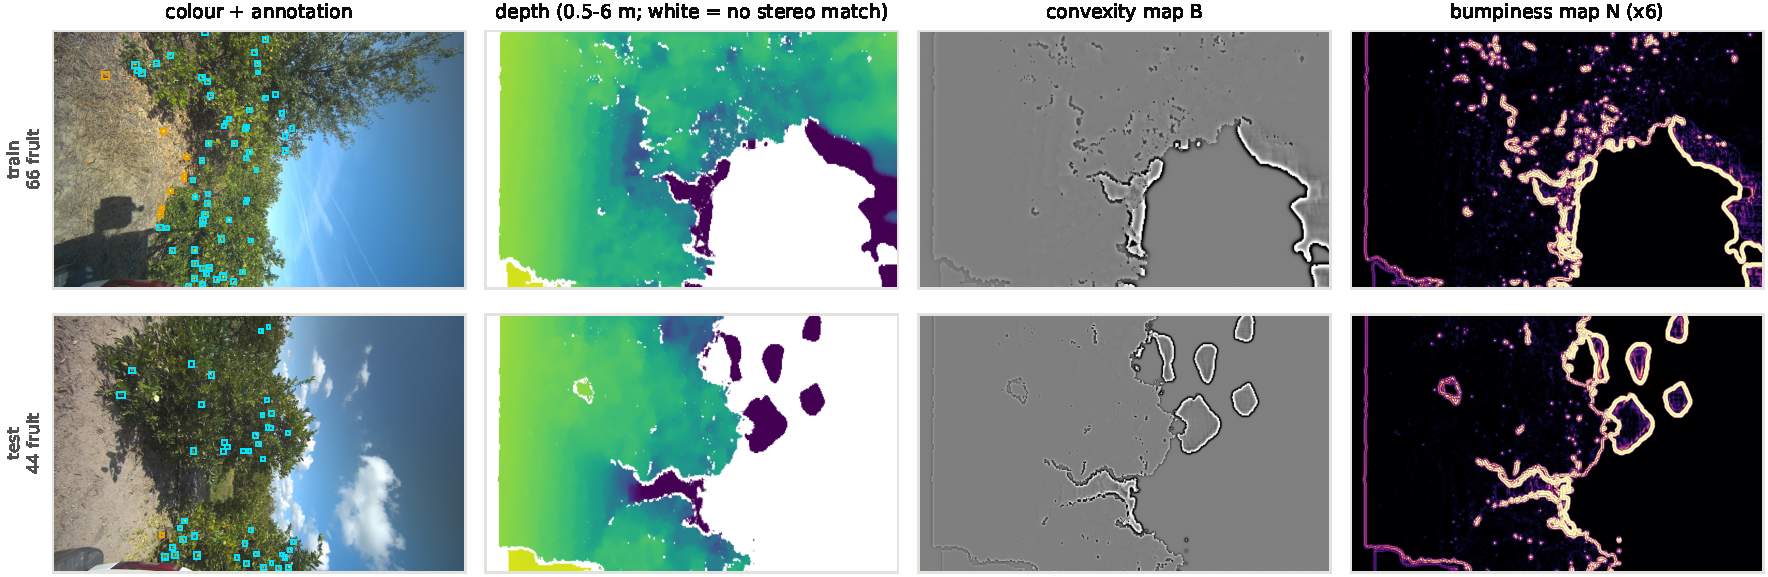
\includegraphics[width=0.98\linewidth]{../figures/fig_data_modalities.pdf}
\caption{复杂外观与不完整几何观测构成果园检测的双重困难。训练与留出果园示例依次给出 RGB、深度及 B／N 曲率图；B 表示凸性，N 表示起伏度。存储图像旋转了 90 度。}
\label{fig:mod}
\end{figure}
图~\ref{fig:mod} 展示了 SOAD 保留局部视觉证据的任务依据。枝叶与果实颜色接近，遮挡区域中的可见边缘和实例间隔成为重要判别线索；深度缺失及枝叶上的曲率响应则使几何信息的价值具有区域差异。原生像素图块将这些可见细节保留至检测输入，几何对照进一步评价额外观测的作用。这些场景特征支持本文优先组织 RGB 局部输入、再检验几何补充信息的设计顺序。
\begin{figure}[H]
\centering
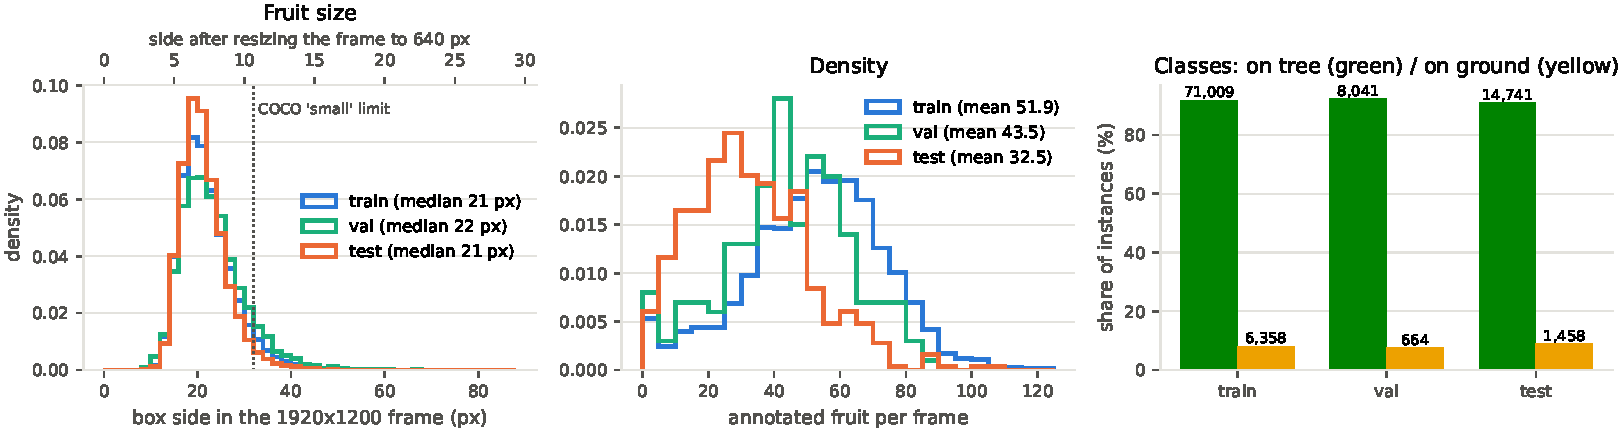
\includegraphics[width=0.98\linewidth]{../figures/fig_data_size_density.pdf}
\caption{小尺寸与密集实例使整图缩放进一步压缩可用观测。各划分的果实尺寸、密度和类别比例，以及整图缩至 640 像素宽时的对应目标尺寸。}
\label{fig:size}
\end{figure}
图~\ref{fig:size} 将输入组织的必要性落实到目标尺度与实例密度。各划分的果实边长中位数约为 21--22 像素，训练图像平均包含 51.9 个果实；整图宽度缩至三分之一时，中位目标边长约为 7 像素，框覆盖面积相应缩至约九分之一。单果外观与相邻实例间隔同时受到压缩，使保留局部采样成为密集检测的重要设计要求。该分布为 SOAD 的原生像素图块方案提供任务依据，其实际收益由分尺寸召回率和整图检测结果进一步验证。
\begin{figure}[H]
\centering
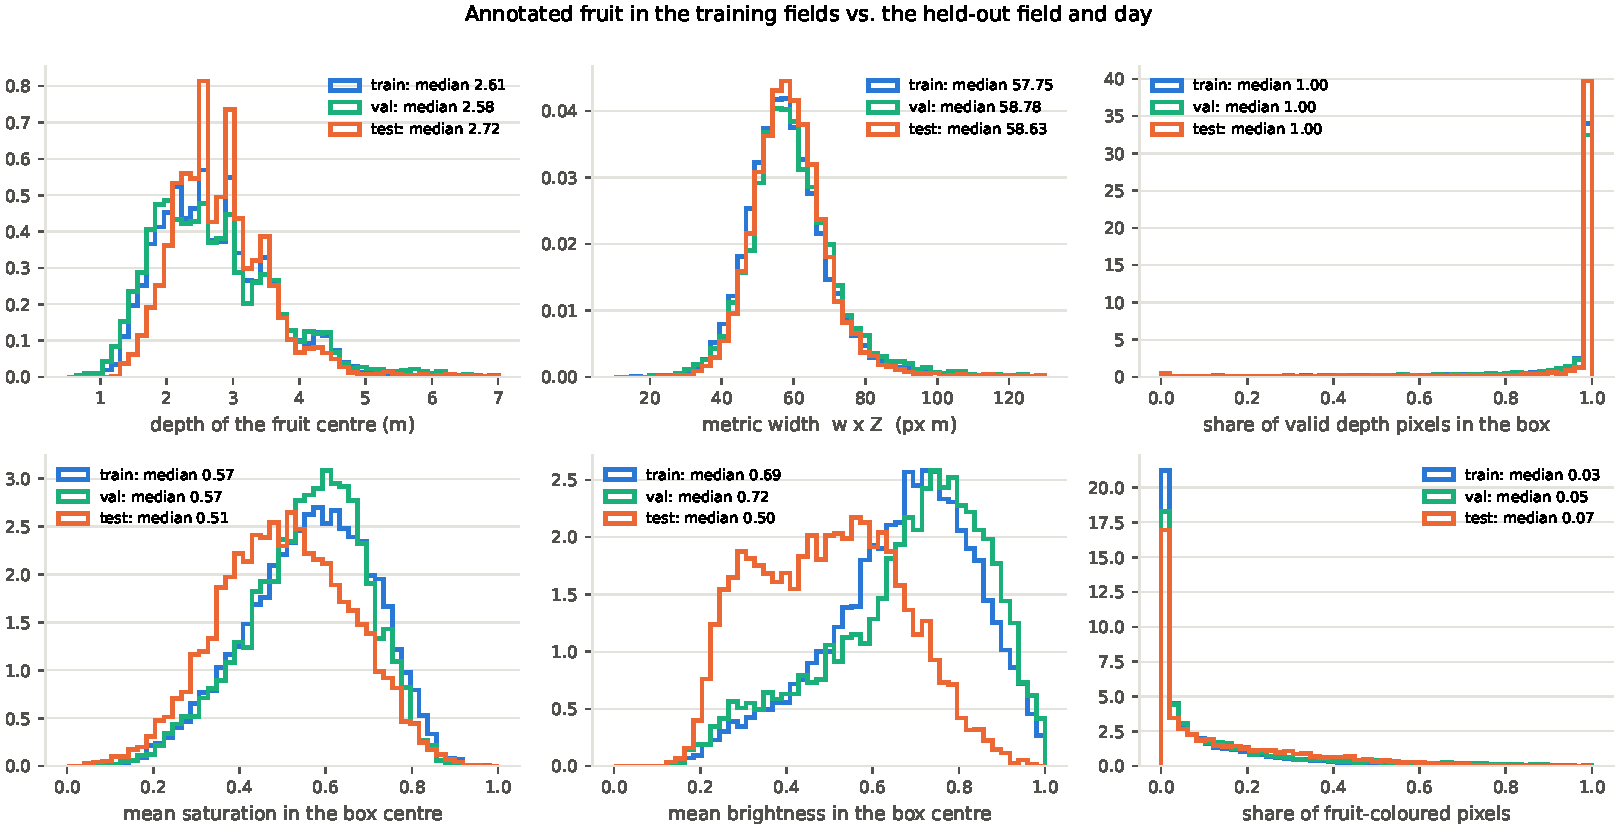
\includegraphics[width=0.98\linewidth]{../figures/fig_data_domain_shift.pdf}
\caption{留出果园同时具有与训练集接近的尺度代理量和不同的颜色统计。比较中心深度、宽度乘深度、有效深度比例与颜色分布；尺度代理量以像素米计，未换算为真实物理宽度。}
\label{fig:shift}
\end{figure}
图~\ref{fig:shift} 表明，留出果园主要增加了外观变化下的检测难度。宽度乘深度的尺度代理量中位数从 57.75 变为 58.63 像素米，相对变化约 1.5\%；亮度中位数从 0.69 变为 0.50，饱和度从 0.57 变为 0.51。接近的尺度代理量与变化的颜色统计，使测试同时考察局部结构识别和跨场景候选筛选。结合后续留出集的精度与计数改善，这一数据条件为 SOAD 的局部输入组织和证据校准在跨果园场景中的有效性提供了评价基础。

所有模型使用同一离线评估器，在整图坐标上按公开实现的匹配与 AP 规则评价。除 mAP50 和 mAP50:95 外，还报告置信度 0.25、IoU 0.5 下的召回率及每图误检数（FPPI），并分别在召回率 0.70 和 0.80 时比较 FPPI。逐图计数误差为置信度 0.25 下检测数与标注数之差的绝对值均值。模型与校准参数均由验证集选择，留出果园仅用于最终评估。统计区间按图像配对重采样 1,000 次，反映图像抽样波动，不覆盖训练随机种子的变异。

\subsection{输入对齐与尺度诊断}
几何分支的效果只有在 RGB 与曲率图像素对齐时才有可解释性。对齐探针用每幅 RGB 图像的灰度版本替换几何图；两路输入经历同一几何增强后，应保留较高的像素相关性。训练预算比较则以网络更新次数为准，图块训练十轮约 18,490 次更新，整图训练一百轮约 18,700 次更新。

\begin{figure}[H]
\centering
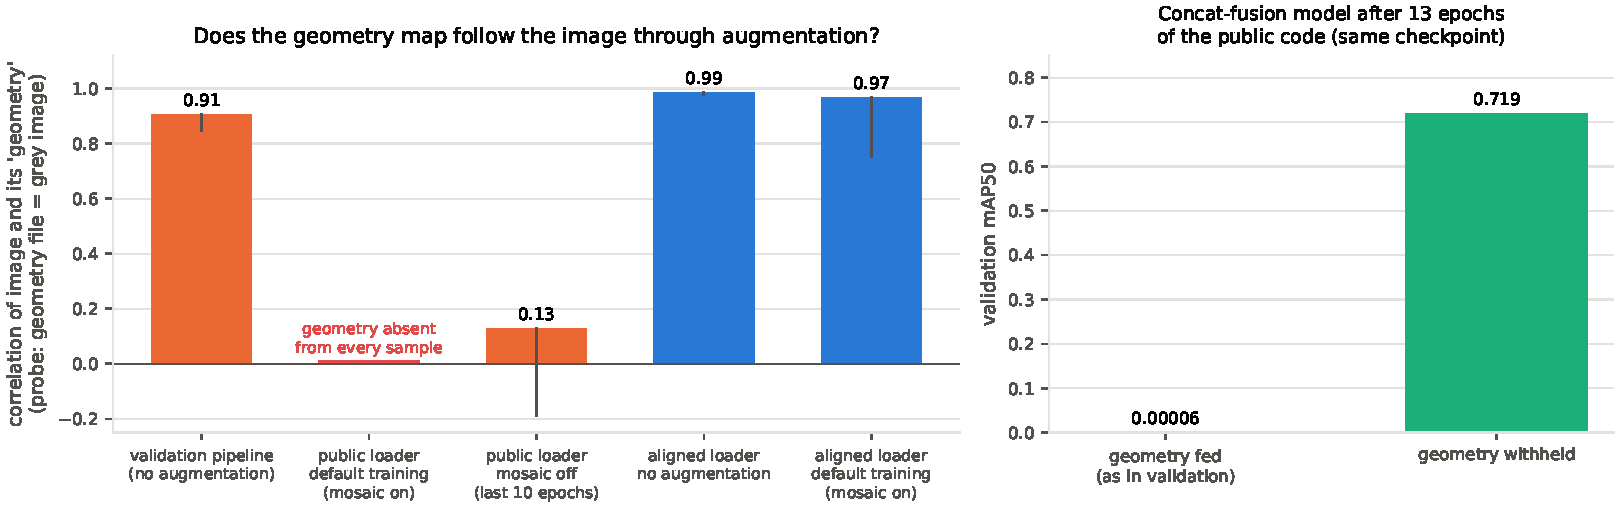
\includegraphics[width=0.98\linewidth]{../figures/fig_alignment.pdf}
\caption{同步增强保持模态间空间对应关系。左侧以 RGB 灰度图替代几何输入进行对齐探针检验；右侧为同一拼接融合检查点保留或撤去异常几何输入时的检测结果。}
\label{fig:align}
\end{figure}
图~\ref{fig:align} 验证了同步增强对空间对应关系的保持作用。灰度探针与 RGB 输入的相关系数由 0.13 提高至 0.97；作为对照，默认分离加载在抽查的 40 个马赛克样本中均丢失几何输入。拼接融合模型撤去异常几何输入后，mAP50 从近零恢复至 0.719，进一步表明输入组织直接影响融合模块获得的有效观测。同步增强因而为本文条件化几何分析提供了可靠的输入基础，使几何对照建立在明确的像素对应关系上。
\begin{figure}[H]
\centering
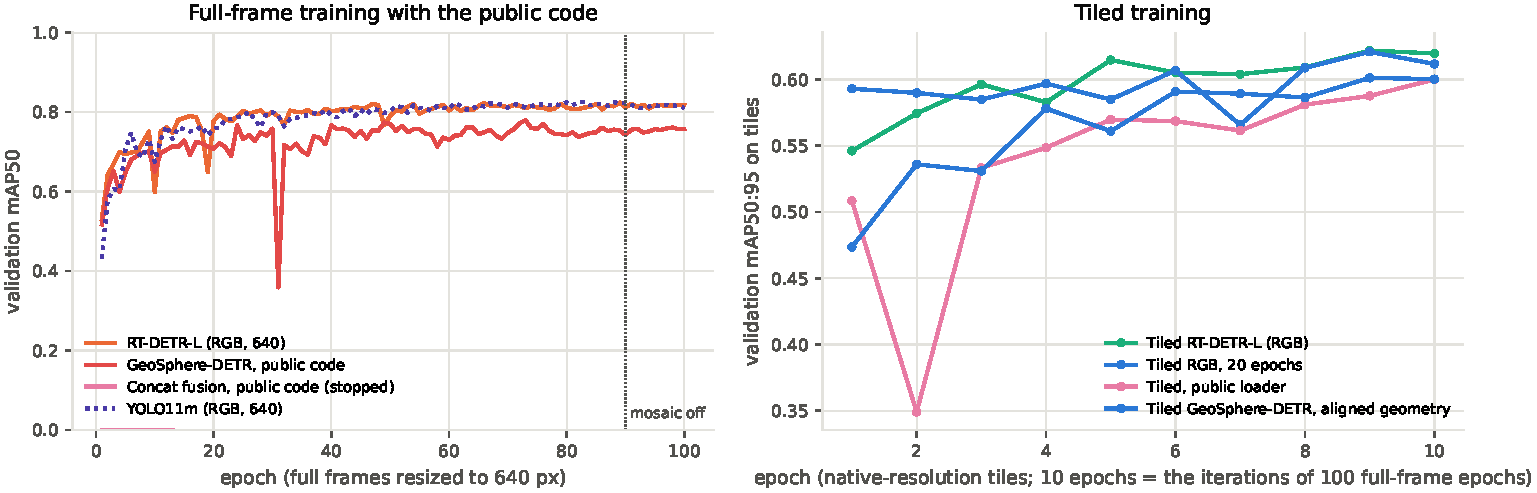
\includegraphics[width=0.98\linewidth]{../figures/fig_training_curves.pdf}
\caption{相近更新预算下的整图与图块训练趋势。左侧使用 mAP50，右侧使用 mAP50:95，曲线高度不直接比较；十轮图块训练与一百轮整图训练的更新次数接近。}
\label{fig:curves}
\end{figure}
图~\ref{fig:curves} 展示了 SOAD 在相近参数更新预算下的训练进程。整图与图块训练分别约为 18,700 和 18,490 次更新，差异约 1.1\%；两条曲线分别描述 mAP50 与 mAP50:95 的训练趋势，最终精度采用表~\ref{tab:main} 的统一指标比较。在这一预算条件下，图块配置取得更高的留出集精度，说明将更新用于原生像素局部样本能够获得有效的检测增益。该结果支持 SOAD 将输入组织纳入训练设计的作用。

在本文数据、RT-DETR-L 骨干与训练预算下，图块输入贡献了各项改动中最大的精度增量。它同时调整目标像素尺度、局部上下文、训练样本组成和推理次数，所测收益对应这一完整输入流程。相近迭代预算下的检测精度与同召回率误检共同改善，为本文从观测组织出发设计检测流程提供实证支持。

\subsection{主要检测性能及误检工作点}
表~\ref{tab:main} 比较 SOAD 与已有同协议实测结果的 RT-DETR-L（2024）\cite{rtdetr}、YOLO11m（2024）\cite{yolo11} 和 GeoSphere-DETR（2026）\cite{geosphere}。SOAD 的 RGB 主路径由验证集镜像融合 mAP50:95 选定。SOAD 模块消融见表~\ref{tab:configs}，几何模型的配对差异见表~\ref{tab:geometry_stats}。

\begin{table}[H]
\centering
\scriptsize\setlength{\tabcolsep}{2.1pt}
\caption{SOAD 与已完成实测的近期方法比较。全部结果来自同一留出果园的 499 幅图像、16,199 个果实及同一整图评估器。}
\label{tab:main}
\begin{tabular}{lrrrrrrr}
\toprule
方法／配置 & mAP50$\uparrow$ & mAP50:95$\uparrow$ & FPPI$\downarrow$ & 召回率$\uparrow$ & \shortstack{FPPI@\\R.70$\downarrow$} & \shortstack{FPPI@\\R.80$\downarrow$} & \shortstack{计数\\误差$\downarrow$} \\
\midrule
RT-DETR-L (2024) \cite{rtdetr} & 0.697 & 0.432 & 53.17 & 0.843 & 9.57 & 23.66 & 48.8 \\
YOLO11m (2024) \cite{yolo11} & 0.640 & 0.391 & 12.44 & 0.690 & 13.69 & 37.97 & 5.7 \\
GeoSphere-DETR (2026) \cite{geosphere} & 0.677 & 0.419 & 23.50 & 0.790 & 9.53 & 26.19 & 16.8 \\
\midrule
\textbf{SOAD（12 次推理）} & 0.813 & 0.566 & 7.60 & 0.844 & 2.35 & 5.32 & 4.5 \\
\textbf{Ours (SOAD，24 次推理)} & \textbf{0.824} & \textbf{0.576} & \textbf{7.37} & \textbf{0.946} & \textbf{2.18} & \textbf{5.24} & \textbf{4.4} \\
\bottomrule
\end{tabular}
\par\vspace{2pt}\parbox{0.97\linewidth}{\footnotesize 方法名后列出发表或发布年份及引用；YOLO11 引用官方发布文档。前三行采用整图缩放输入，每图执行 1 次网络推理。SOAD 名称中的次数表示每幅图像的 640 像素网络推理次数。12 次配置保留证据校准、关闭镜像融合，对应表~\ref{tab:configs} 的 w/o MF；24 次配置为根据验证集选定的完整 SOAD。两种 SOAD 配置均采用图块输入。粗体表示本表各性能列的最优值，$\uparrow/\downarrow$ 分别表示越高／越低越好。FPPI、召回率和计数误差使用置信度 0.25，FPPI@R 使用固定召回率。}
\end{table}
表~\ref{tab:main} 表明，SOAD 将输入组织与输出处理结合后，实现了跨果园检测精度和同召回率误检的共同改善。相对整图 RT-DETR-L，mAP50:95 提高 14.4 个百分点，FPPI@R.70 从 9.57 降至 2.18，减少约 77.2\%；对应 mAP50:95 配对检验为 $p<0.001$（表~\ref{tab:ladder}）。这一统计显著的精度增益支持 SOAD 完整流程的有效性。两种配置分别执行 1 次与 24 次网络推理，性能差异对应不同的输入和计算配置。

另在匹配图块和附加处理的对照中，SOAD 的 FPPI@R.70 和 FPPI@R.80 均低于几何模型，支持其在高召回率条件下控制背景误检的作用。几何对照的 mAP50:95 为 0.580，高于 SOAD 的 0.576，固定阈值 FPPI 与计数误差也更低；两者的 mAP50:95 差值区间为 $-0.001$ 至 $+0.009$，$p=0.100$，见表~\ref{tab:geometry_stats} 与图~\ref{fig:ladder}。这一结果界定了两种方法各自的性能特点，SOAD 的正向证据集中于同召回率误检及相对整图基线的整体提升。主配置由验证集选定，统计比较评价固定权重下的图像抽样差异。

\begin{figure}[H]
\centering
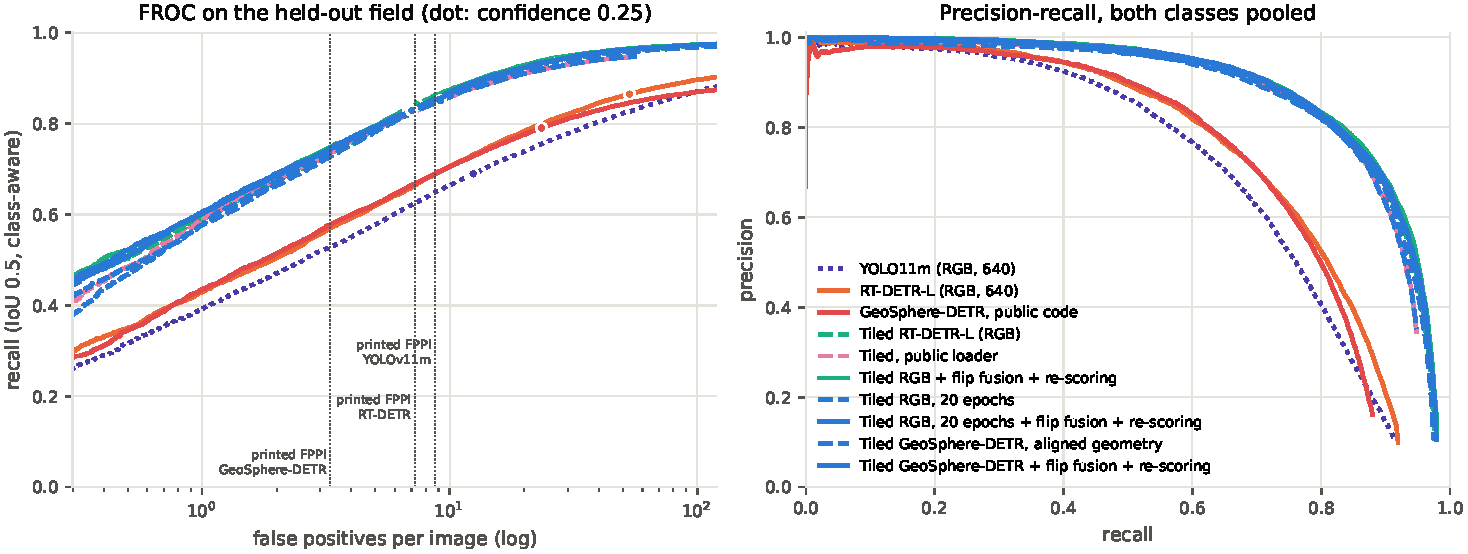
\includegraphics[width=0.98\linewidth]{../figures/fig_froc_pr.pdf}
\caption{图块输入的检测优势覆盖多个置信度工作点。FROC 与精确率--召回率曲线中，圆点表示置信度 0.25；文献误检率竖线因缺少对应召回率，仅供参照。}
\label{fig:froc}
\end{figure}
图~\ref{fig:froc} 将 SOAD 相对整图基线的改善扩展到多个置信度工作点。图块模型的 FROC 曲线在较宽误检范围内位于整图模型上方，表明给定误检预算时能够检出更多果实；高召回区的 PR 曲线则体现了候选筛选的有效性。校准前后曲线接近而固定阈值工作点发生移动，说明证据校准能够调整实际保留的候选集合。该结果从连续工作点上支持输入组织与输出校准的分工，使完整流程的收益同时体现为检出能力和输出可用性的改善。

几何对照进一步说明了统一召回率评价的作用。在置信度 0.25 下，图块 RGB 模型与对齐几何模型的召回率分别为 0.943 和 0.851，FPPI 分别为 30.87 和 9.18；固定召回率为 0.70 后，FPPI 分别为 2.49 和 2.45。统一工作点将误检控制与候选保留比例区分开来，为评价 SOAD 校准模块提供明确依据。验证集镜像融合后的 RGB 与几何模型 mAP50:95 分别为 0.643 和 0.639，支持采用验证集选定的十轮 RGB 检测主路径。

\begin{figure}[H]
\centering
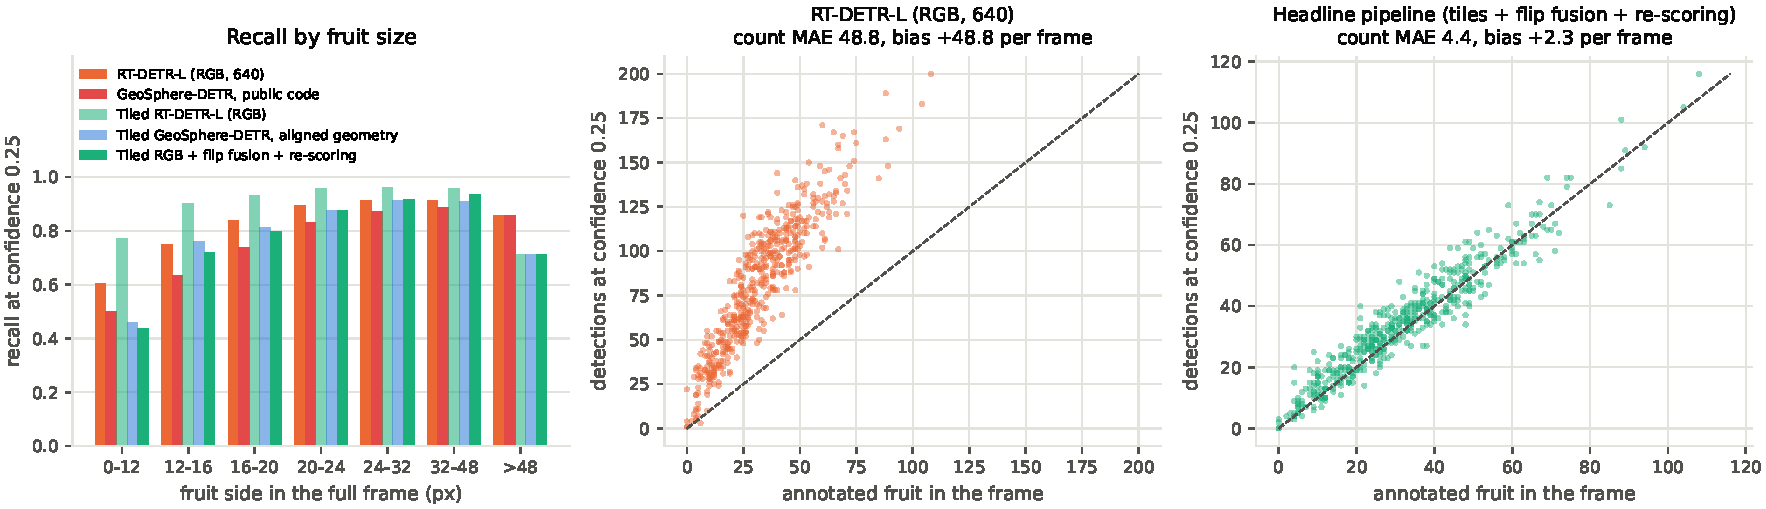
\includegraphics[width=0.98\linewidth]{../figures/fig_size_count.pdf}
\caption{小果实检出与整图计数共同改善。左侧为置信度 0.25 下的分尺寸召回率，中间和右侧为整图基线与完整 SOAD 的预测数量及标注数量。}
\label{fig:count}
\end{figure}
图~\ref{fig:count} 将小果实检出增益与整图计数质量联系起来。图块 RGB 模型在多数小尺寸组具有更高召回率，支持原生像素输入对困难小目标的检出作用；完整 SOAD 的预测数量更接近标注数量，计数平均绝对误差由整图基线的 48.8 降至 4.4，降低约 91.0\%，平均多检偏差从 48.8 降至 2.3。该结果表明，局部输入保留、整图实例聚合和证据校准能够共同把检测改善转化为更准确的果实数量估计，直接支撑 SOAD 面向检测与计数的整体设计。

\begin{figure}[H]
\centering
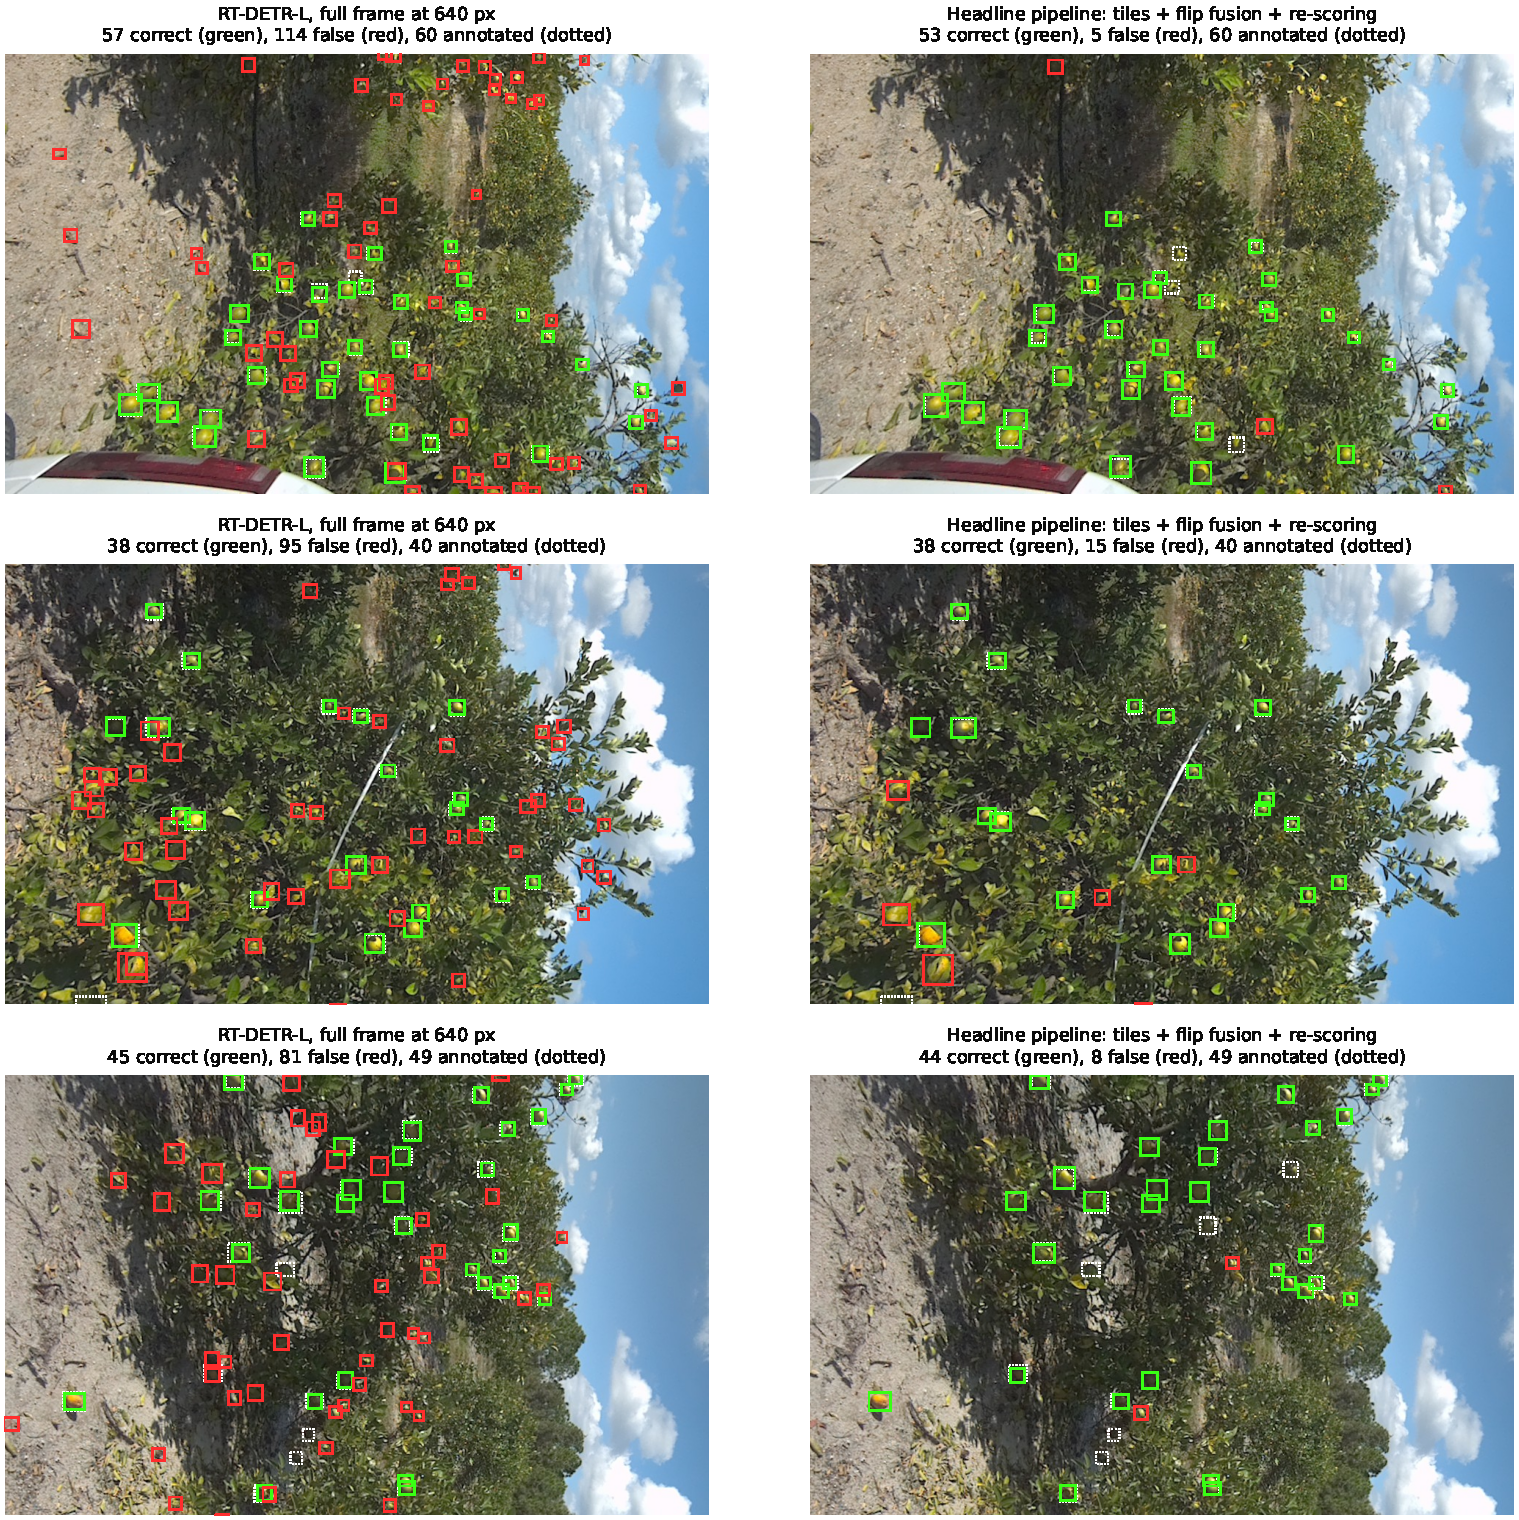
\includegraphics[width=0.98\linewidth]{../figures/fig_qualitative.pdf}
\caption{完整 SOAD 在所示困难背景中明显减少误检。左侧为整图 RT-DETR-L，右侧为 SOAD；绿色框为 IoU 0.5 下的正确检测，红色框为误检，白色虚线框为标注。}
\label{fig:qual}
\end{figure}
图~\ref{fig:qual} 展示了 SOAD 对黄叶、亮土和反光背景的筛选效果。三例误检分别减少约 95.6\%、84.2\% 和 90.1\%，正确检测框数分别保留整图基线的约 93.0\%、100\% 和 97.8\%。在保留大部分正确检测的同时明显减少错误框，表明完整流程能够有效区分所示背景响应与真实果实。这些案例为 SOAD 的候选筛选设计提供直观支持，并与全测试集的同召回率误检下降和计数改善相互印证。

本文以 RT-DETR-L、YOLO11m 和 GeoSphere-DETR 为独立实测基线，统一数据划分、有效测试样本与整图评估器。方法间结论对应这三项基线及表~\ref{tab:main} 所列输入和计算配置。

\subsection{组件贡献与证据重新评分}
本节检验 SOAD 的输入组织、镜像融合与证据校准。表~\ref{tab:configs} 以移除模块的方式定义 SOAD 变体；几何模型比较见表~\ref{tab:main}。

\begin{table}[H]
\centering
\scriptsize\setlength{\tabcolsep}{2.1pt}
\caption{SOAD 输出模块消融。四组采用同一十轮训练检查点、原生像素图块及跨块聚合，仅切换镜像融合与证据校准。}
\label{tab:configs}
\begin{tabular}{lrrrrrrrr}
\toprule
方法变体 & 推理量 & mAP50$\uparrow$ & mAP50:95$\uparrow$ & FPPI$\downarrow$ & 召回率$\uparrow$ & \shortstack{FPPI@\\R.70$\downarrow$} & \shortstack{FPPI@\\R.80$\downarrow$} & \shortstack{计数\\误差$\downarrow$} \\
\midrule
\textbf{SOAD} w/o MF \& EC & 12 & 0.812 & 0.567 & 30.87 & 0.943 & 2.49 & 5.29 & 29.0 \\
\textbf{SOAD} w/o MF & 12 & 0.813 & 0.566 & 7.60 & 0.844 & 2.35 & 5.32 & 4.5 \\
\textbf{SOAD} w/o EC & 24 & 0.819 & 0.574 & 29.22 & 0.865 & 2.35 & 5.27 & 27.5 \\
\midrule
\textbf{Ours (SOAD)} & 24 & \textbf{0.824} & \textbf{0.576} & \textbf{7.37} & \textbf{0.946} & \textbf{2.18} & \textbf{5.24} & \textbf{4.4} \\
\bottomrule
\end{tabular}
\par\vspace{2pt}\parbox{0.97\linewidth}{\footnotesize MF 表示镜像融合（Mirror Fusion），EC 表示证据校准（Evidence Calibration）；w/o 表示移除对应环节。粗体为本表各性能列最优值；推理量及各指标定义同表~\ref{tab:main}。}
\end{table}
表~\ref{tab:configs} 为镜像融合与证据校准的组合提供直接消融证据。镜像融合使基础配置的 mAP50:95 从 0.567 提高至 0.574；仅加入校准时，计数误差从 29.0 降至 4.5，对应 mAP50:95 为 0.566。完整 SOAD 达到 0.576 mAP50:95、2.18 FPPI@R.70 和 4.4 计数误差，三项均优于单模块配置。该结果支持将镜像定位证据与候选质量校准组合使用，使精度提升与数量估计改善在同一流程中实现。



表~\ref{tab:ladder} 以留出图像为单位进行配对自助法重采样，检验输入组织、镜像融合和校准在逐步组合过程中的性能增量。统计分析固定模型权重，量化测试图像抽样引起的波动。

\begin{table}[H]
\centering
\scriptsize\setlength{\tabcolsep}{1.1pt}
\caption{SOAD 输入组织与输出模块的配对性能增量。按留出图像重采样 1,000 次，括号内为 95\% 区间。}
\label{tab:ladder}
\begin{tabular}{>{\raggedright\arraybackslash}p{4.6cm}lllc}
\toprule
比较 & $\Delta$ mAP50 & $\Delta$ mAP50:95 & $\Delta$ FPPI（置信度 0.25） & $p$ \\
\midrule

整图 RT-DETR-L $\rightarrow$ \textbf{SOAD} w/o MF \& EC & +0.115 (+0.104 至 +0.125) & +0.134 (+0.126 至 +0.142) & $-$22.3 ($-$23.5 至 $-$21.2) & $<$0.001 \\
恢复 MF（固定无 EC） & +0.007 (+0.004 至 +0.009) & +0.007 (+0.005 至 +0.009) & $-$1.7 ($-$1.9 至 $-$1.4) & $<$0.001 \\
恢复 EC（固定启用 MF） & +0.005 (+0.003 至 +0.007) & +0.002 (+0.001 至 +0.004) & $-$21.9 ($-$22.8 至 $-$21.0) & 0.002 \\
整图 RT-DETR-L $\rightarrow$ \textbf{SOAD（完整配置）} & \textbf{+0.126} (+0.116 至 +0.137) & \textbf{+0.144} (+0.136 至 +0.151) & $\mathbf{-45.8}$ ($-$47.6 至 $-$44.1) & $<$0.001 \\






\bottomrule
\end{tabular}
\par\vspace{2pt}\parbox{0.97\linewidth}{\footnotesize $p$ 为 mAP50:95 的双侧自助法检验值。涉及重新评分的 FPPI 差值在固定置信度下比较了不同分数尺度；相同召回率下的比较见表~\ref{tab:main}及图~\ref{fig:froc}。粗体标示各差值列的最大精度增量或误检降幅；比较起点不同。}
\end{table}
表~\ref{tab:ladder} 为 SOAD 的逐步组合提供了统计显著的精度证据。图块输入的 mAP50:95 增量为 0.134，95\% 区间为 0.126--0.142；在基础流程上恢复镜像融合，增量为 0.007，区间为 0.005--0.009；在镜像融合后恢复校准，增量为 0.002，区间为 0.001--0.004。对应 $p$ 值分别为 $<0.001$、$<0.001$ 和 0.002，均低于 0.05。这些结果支持原生像素输入承担主要精度提升、镜像融合与证据校准提供进一步增益的组合设计，显著性对应固定权重下的留出图像抽样。

上述统计以固定模型权重为条件，量化留出图像的抽样波动。几何模型之间的差异在独立对照中分析，见表~\ref{tab:geometry_stats}。

为检验检测后校准利用了哪些有效证据，表~\ref{tab:per} 在固定分类与质量回归训练目标的条件下改变特征组，并同时报告验证集折外结果、留出集排序精度和同召回率误检。两项损失在各组中保持一致，组间差异对应输入证据组合的变化。

\begin{table}[H]
\centering
\footnotesize
\caption{校准证据组合对排序精度及同召回率误检的影响。各组均使用 SOAD 镜像融合产生的候选框。}
\label{tab:per}
\begin{tabular}{lrrrr}
\toprule
校准器使用的证据 & 验证集 mAP50:95 & 测试集 mAP50 & 测试集 mAP50:95 & 测试集 FPPI@R \\
\midrule
检测器得分（不重新评分） & \textbf{0.643} & 0.819 & 0.574 & 29.16 \\
\midrule
仅得分 & 0.638 & 0.816 & 0.572 & 30.22 \\
上下文 & 0.640 & 0.817 & 0.572 & 30.24 \\
上下文＋框 & 0.641 & 0.819 & 0.574 & 27.44 \\
上下文＋深度 & 0.641 & 0.817 & 0.572 & 30.41 \\
上下文＋尺寸 & 0.641 & 0.821 & 0.574 & 28.49 \\
上下文＋曲率 & 0.640 & 0.817 & 0.572 & 30.15 \\
上下文＋颜色 & 0.642 & 0.821 & 0.574 & 29.98 \\
全部 $-$ 框 & 0.642 & \textbf{0.824} & \textbf{0.576} & 28.14 \\
全部 $-$ 深度 & 0.642 & 0.823 & \textbf{0.576} & \textbf{26.74} \\
全部 $-$ 尺寸 & 0.642 & 0.823 & 0.575 & 27.38 \\
全部 $-$ 曲率 & 0.642 & 0.823 & \textbf{0.576} & 27.04 \\
全部 $-$ 颜色 & 0.640 & 0.821 & 0.575 & 26.99 \\
\textbf{全部（SOAD 完整校准）} & 0.642 & \textbf{0.824} & \textbf{0.576} & 27.12 \\
\bottomrule
\end{tabular}
\par\vspace{2pt}\parbox{0.97\linewidth}{\footnotesize 验证集结果采用按图像分组的折外预测。FPPI@R 表示检测器在置信度 0.25 所对应召回率下的每图误检数。上下文包含检测得分、类别、排名和图内框重叠。特征组包括框几何、深度、物理尺寸、曲率图和颜色。粗体为各列最优值，并列均标出；FPPI 越低越好。}
\end{table}
表~\ref{tab:per} 支持在候选得分之外引入上下文与框相关证据。完整组合相对仅得分配置将测试集 mAP50:95 从 0.572 提高至 0.576；相对上下文配置，FPPI@R 从 30.24 降至 27.12，减少约 10.3\%。与不重新评分的检测器相比，完整校准在相同召回率下减少约 7.0\% 的误检，并增加 0.002 的 mAP50:95。上述增益为 SOAD 的检测后证据校准提供直接支持，表明补充候选描述能够改善输出排序与筛选。

特征消融进一步明确了有效证据的来源。上下文中加入框特征后，FPPI@R 从 30.24 降至 27.44，支持将空间描述用于候选可信度估计。完整配置移除深度或曲率后仍为 0.576 mAP50:95，其中去掉深度的 FPPI@R 为 26.74，完整组合为 27.12；验证集折外 mAP50:95 分别为未校准 0.643、完整校准 0.642。各证据组合呈现不同工作点表现，本文以固定联合训练目标下的特征消融解释校准输入的贡献。其对方法设计的支持在于明确框与上下文证据的价值，并为输入证据的选择提供依据。
\begin{figure}[H]
\centering
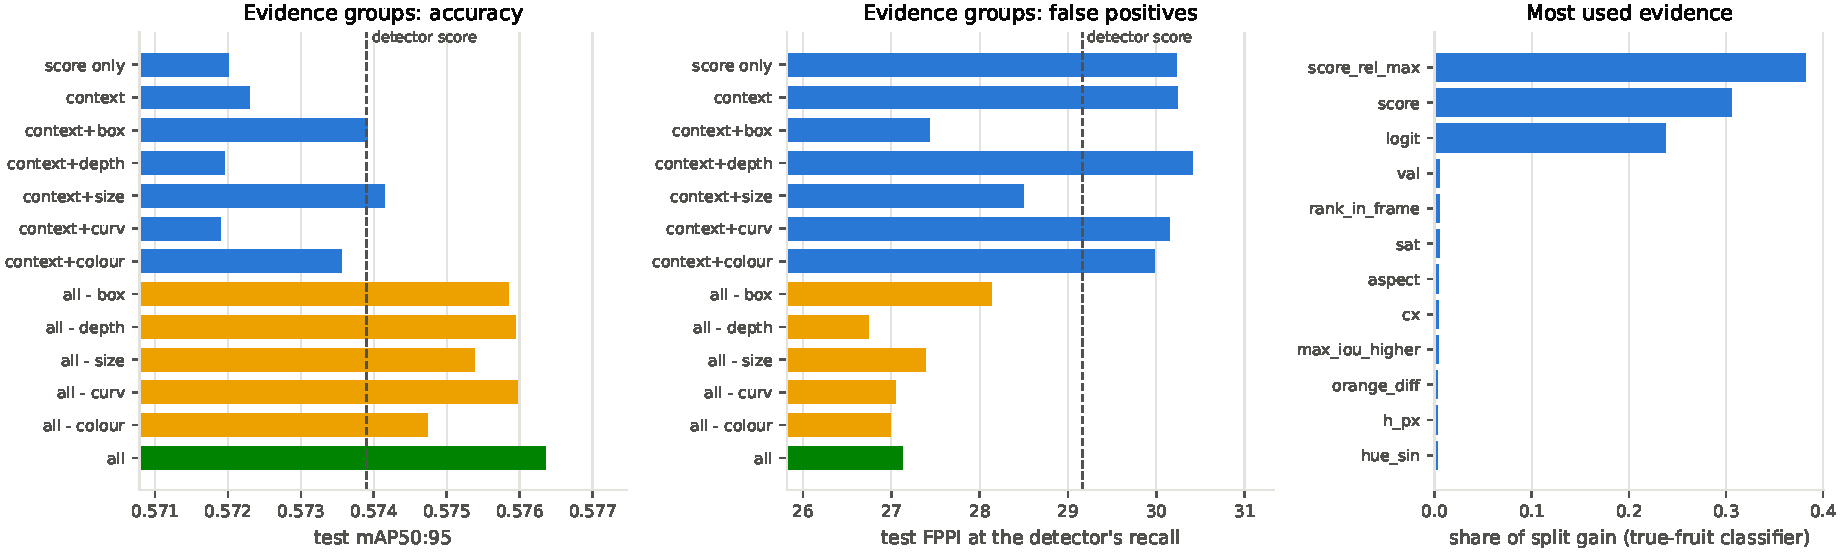
\includegraphics[width=0.98\linewidth]{../figures/fig_rescoring_ablation.pdf}
\caption{完整证据组合改善校准结果，分类器主要依赖检测置信信息。依次给出特征组消融的精度、原召回率下误检及真果分类器的特征重要性。}
\label{fig:per}
\end{figure}
图~\ref{fig:per} 从性能变化和特征使用两个方面解释证据校准的作用。相对得分、原始得分及其对数值占据主要分裂增益，表明校准器以检测置信信息为基础组织判断；完整证据相对仅得分配置同时提高 mAP50:95 并降低同召回率误检，说明补充候选描述具有实际价值。特征重要性描述模型使用的证据，移除对照检验这些证据对性能的影响，两者共同支持在冻结检测器之后学习候选质量的模块设计。

\subsection{与几何检测方法的受控比较}
本节通过配对统计分析检测方法与几何输入条件的差异，并结合图~\ref{fig:ladder} 展示输入组织和输出处理的性能增量。

\begin{table}[H]
\centering
\scriptsize\setlength{\tabcolsep}{1.1pt}
\caption{检测方法与几何输入条件的配对差异。按留出图像重采样 1,000 次，括号内为 95\% 区间。}
\label{tab:geometry_stats}
\begin{tabular}{>{\raggedright\arraybackslash}p{4.6cm}lllc}
\toprule
比较 & $\Delta$ mAP50 & $\Delta$ mAP50:95 & $\Delta$ FPPI（置信度 0.25） & $p$ \\
\midrule
整图 RT-DETR-L $\rightarrow$ GeoSphere-DETR（统一协议） & $-$0.021 ($-$0.030 至 $-$0.011) & $-$0.013 ($-$0.020 至 $-$0.007) & $\mathbf{-29.7}$ ($-$30.9 至 $-$28.5) & $<$0.001 \\




整图 GeoSphere-DETR$\rightarrow$ \textbf{SOAD（完整配置）} & \textbf{+0.147} (+0.134 至 +0.159) & \textbf{+0.157} (+0.148 至 +0.165) & $-$16.1 ($-$16.9 至 $-$15.4) & $<$0.001 \\
切块 RGB $\rightarrow$ 切块 GeoSphere-DETR（几何图对齐） & $-$0.009 ($-$0.018 至 +0.000) & $-$0.003 ($-$0.009 至 +0.004) & $-$21.7 ($-$22.5 至 $-$20.9) & 0.472 \\
上述比较，均加入翻转融合与重新评分 & +0.002 ($-$0.005 至 +0.009) & +0.004 ($-$0.001 至 +0.009) & $-$0.4 ($-$0.5 至 $-$0.2) & 0.100 \\
切块 GeoSphere-DETR 加载器对齐前后 & $-$0.004 ($-$0.012 至 +0.004) & +0.002 ($-$0.004 至 +0.008) & $-$1.3 ($-$1.5 至 $-$1.1) & 0.594 \\

切块 GeoSphere-DETR 640 像素输入与 960 像素微调 & $-$0.006 ($-$0.016 至 +0.003) & $-$0.010 ($-$0.018 至 $-$0.003) & +1.5 (+1.2 至 +1.7) & 0.002 \\
\bottomrule
\end{tabular}
\par\vspace{2pt}\parbox{0.97\linewidth}{\footnotesize $p$ 为 mAP50:95 的双侧自助法检验值。涉及重新评分的 FPPI 差值在固定置信度下比较了不同分数尺度；相同召回率下的比较见表~\ref{tab:main}及图~\ref{fig:froc}。粗体标示各差值列的最大精度增量或误检降幅；比较起点不同。}
\end{table}
表~\ref{tab:geometry_stats} 从另一条整图基线验证了 SOAD 完整流程的收益。相对整图 GeoSphere-DETR，SOAD 的 mAP50:95 增量为 0.157，95\% 区间为 0.148--0.165，$p<0.001$，为输入组织与输出处理共同带来的精度提升提供统计支持。匹配图块条件下，几何模型相对 RGB 模型的单视图和完整处理增量分别为 $-0.003$ 与 $+0.004$，区间均包含零，体现了几何收益随观测和处理条件变化的特点。这一对照落实了本文按既定输入条件评价额外几何信息的分析框架，同时将整体流程增益与模型间较小差异分别量化。


\begin{figure}[H]
\centering
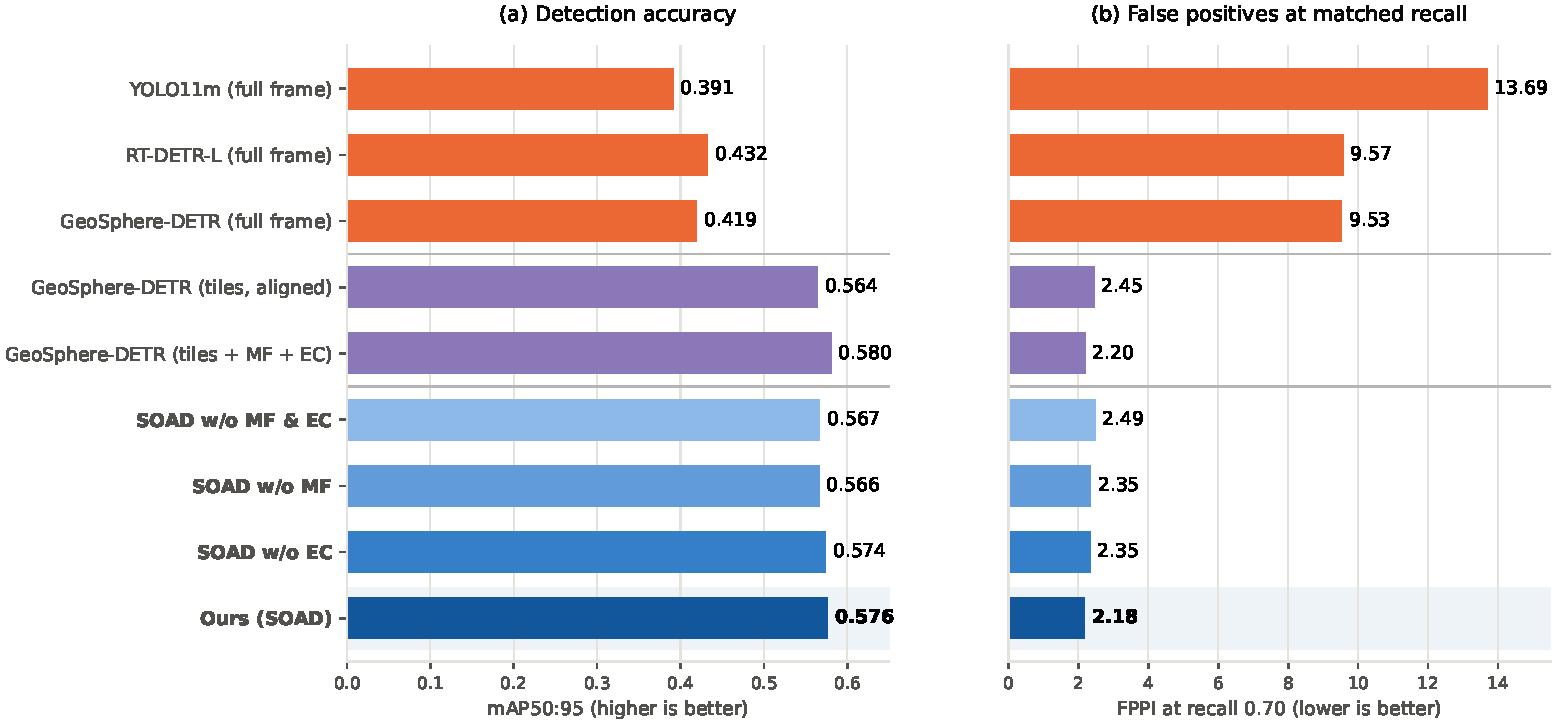
\includegraphics[width=0.98\linewidth]{../figures/fig_ladder.pdf}
\caption{SOAD 输入组织与输出模块的性能增量。橙色为整图基线，紫色为采用对齐图块的几何对照，蓝色为 SOAD 变体；完整 SOAD 位于最下方并加粗。左图比较 mAP50:95，右图在召回率 0.70 下比较每图误检数。MF 为镜像融合，EC 为证据校准。全部数值来自同一留出集实测。}
\label{fig:ladder}
\end{figure}
图~\ref{fig:ladder} 清晰呈现 SOAD 从局部输入到实例输出的增益分配。基础 SOAD 相对整图 RT-DETR-L 增加 0.135 mAP50:95，占完整流程总增量 0.144 的约 94\%，FPPI@R.70 同时从 9.57 降至 2.49，表明图块训练与实例聚合构成主要性能来源。单独加入镜像融合的 mAP50:95 为 0.574，单独加入校准为 0.566，两者的 FPPI@R.70 均为 2.35；完整组合进一步达到 0.576 和 2.18。该结果支持镜像融合侧重提高检测精度、证据校准侧重优化候选筛选的功能分工，并验证两者组合对完整输出质量的提升。

几何图块对照在相同处理条件下补充验证了 SOAD 的误检控制特点。几何模型的完整配置为 0.580 mAP50:95，SOAD 为 0.576；两者的 FPPI@R.70 分别为 2.20 和 2.18。SOAD 在该工作点取得更低的误检数，为其背景筛选作用提供补充证据。图~\ref{fig:ladder} 展示性能变化的方向与幅度，表~\ref{tab:ladder} 和表~\ref{tab:geometry_stats} 则给出对应统计分析。

\subsection{计算代价}

几何模型的尺度对照为采用原生 640 像素图块提供了配置依据。原生配置的测试集 mAP50:95 为 0.564，高于放大至 960 像素并追加四轮微调后的 0.554；验证集直接放大推理时，mAP50:95 从 0.626 变为 0.545。该对照支持在当前训练条件下保留原生图块尺度，以较低的输入面积取得更高精度；这一结果对应所测试的几何架构。

图块输入保留更多局部像素的同时增加了网络执行次数。图~\ref{fig:cost} 用每幅图像的等效 640 像素推理量表示计算代价，960 像素配置按输入面积折算；该指标不包含图块准备、整图去重、校准特征提取和设备间数据传输时间。

\begin{figure}[H]
\centering
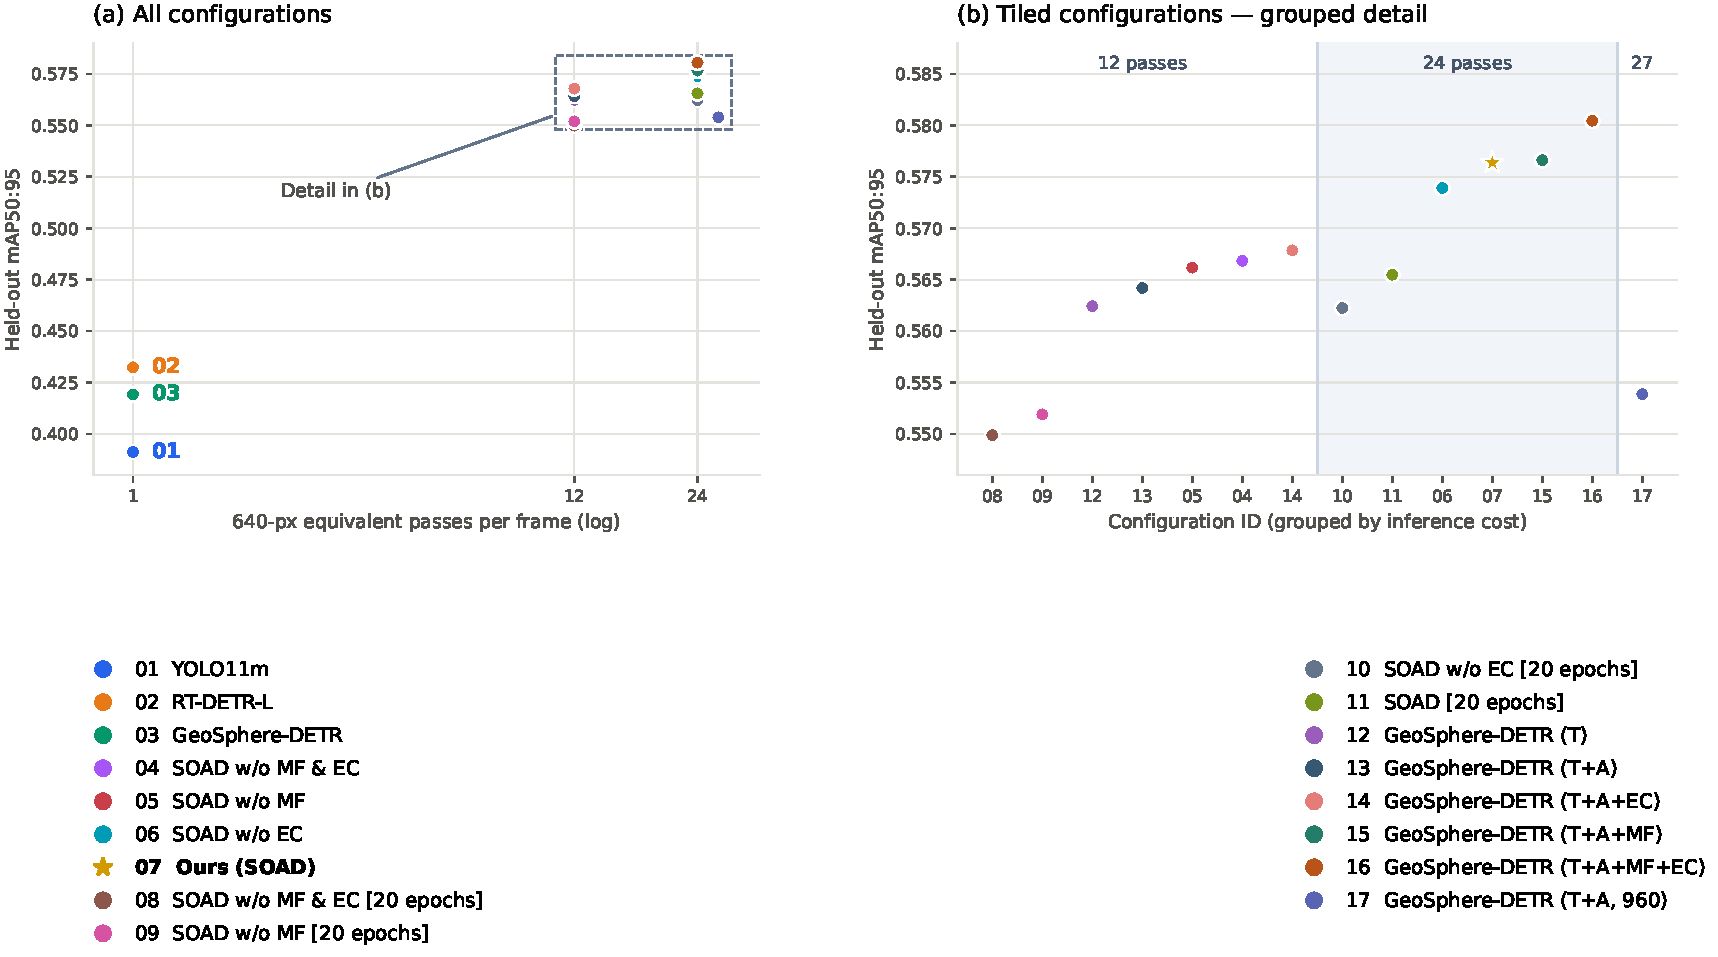
\includegraphics[width=0.98\linewidth]{../figures/fig_cost.pdf}
\caption{检测精度与推理量的关系。（a）全部配置；（b）按推理量分组的图块配置局部放大，横轴为配置编号。每个配置采用独立颜色，编号与下方图例对应，星形表示完整 SOAD。MF、EC、T 和 A 分别表示镜像融合、证据校准、图块输入和同步对齐。640 像素配置按网络调用次数计量，960 像素配置按输入面积折算为 27；推理量不包含校准及数据处理时间。}
\label{fig:cost}
\end{figure}
图~\ref{fig:cost} 显示，SOAD 的基础输入流程能够获得主要精度收益。基础配置执行十二次图块推理，达到 0.567 mAP50:95；完整配置为 0.576，相对 0.432 整图基线的增量中约 94\% 已由基础配置实现。镜像融合进一步增加精度，形成输入组织承担主要提升、输出融合提供附加改善的层次。该结果从精度与推理量两个维度支持 SOAD 的模块化设计，计算量采用网络调用次数及输入面积折算，端到端时延另属设备部署指标。
全部模型采用单个随机种子训练，配对自助法区间量化固定模型权重下的测试图像抽样波动。数据覆盖柑橘及本数据集采用的传感器，跨果园测试评价这一采集条件下的场景迁移。校准器使用训练果园的 200 幅验证图像拟合，其跨园表现由检测排序、同召回率误检和计数误差共同评价。深度与曲率特征的作用以表~\ref{tab:per} 的移除对照为依据。

\section{结论}
本文提出 SOAD，将原生像素图块训练、跨块实例聚合、镜像融合和证据校准组织为完整检测流程。相近训练迭代预算下，基础流程使留出果园 mAP50:95 从整图 RGB 基线的 0.432 提升至 0.567，完整配置达到 0.576；召回率为 0.70 时，FPPI 从 9.57 降至 2.18。配对检验支持完整流程相对整图基线的显著精度提升，模块消融进一步验证镜像融合与证据校准在精度和计数上的互补作用。匹配处理后的几何对照取得 0.580 mAP50:95，SOAD 则具有更低的同召回率误检。实验共同支持从输入观测、实例聚合到候选质量逐层组织密集柑橘检测，其测得收益对应目标尺度、上下文与样本组成共同调整的完整流程。

\section*{数据与代码}
数据集见 \cite{dataset}。本文数值、检测结果、分析脚本和原始图文件来自随文项目目录。各图的图内标识为英文，图题和正文为中文。

\begin{thebibliography}{99}\small
\bibitem{rtdetr} Y. Zhao et al., “DETRs Beat YOLOs on Real-time Object Detection,” \emph{Proc. IEEE/CVF CVPR}, 2024, pp. 16965--16974. \url{https://arxiv.org/abs/2304.08069}
\bibitem{rtdetrv2} W. Lv et al., “RT-DETRv2: Improved Baseline with Bag-of-Freebies for Real-Time Detection Transformer,” arXiv:2407.17140, 2024. \url{https://arxiv.org/abs/2407.17140}
\bibitem{agyolo} Y. Lin et al., “AG-YOLO: A Rapid Citrus Fruit Detection Algorithm with Global Context Fusion,” \emph{Agriculture}, vol. 14, no. 1, 114, 2024. doi:10.3390/agriculture14010114.
\bibitem{mfaf} Y. Zhang et al., “Multi-scale feature adaptive fusion model for real-time detection in complex citrus orchard environments,” \emph{Computers and Electronics in Agriculture}, vol. 219, 108836, 2024. doi:10.1016/j.compag.2024.108836.
\bibitem{yuyolo} Y. Yu et al., “Object Detection Algorithm for Citrus Fruits Based on Improved YOLOv5 Model,” \emph{Agriculture}, vol. 14, no. 10, 1798, 2024. doi:10.3390/agriculture14101798.
\bibitem{geosphere} S. Liu et al., “GeoSphere-DETR: RGB-D citrus fruit detection in cluttered orchards via geometry-gated fusion and geometry-aware confidence recalibration,” \emph{Artificial Intelligence in Agriculture}, 2026. doi:10.1016/j.aiia.2026.08.010.
\bibitem{sahi} F. C. Akyon, S. O. Altinuc, and A. Temizel, “Slicing Aided Hyper Inference and Fine-tuning for Small Object Detection,” \emph{Proc. IEEE ICIP}, 2022, pp. 966--970. doi:10.1109/ICIP46576.2022.9897990.
\bibitem{asahi} F. Moretti, Y. Jin, and G. Mario, “Adaptive Slicing-Assisted Hyper Inference for Enhanced Small Object Detection in High-Resolution Imagery,” arXiv preprint arXiv:2604.19233, 2026. \url{https://arxiv.org/abs/2604.19233}
\bibitem{ciafnet} Y. Chen et al., “CIAFNet: An RGB-D Cross-Modal Interaction and Adaptive Fusion Network for Camellia oleifera Fruit Detection,” \emph{Agriculture}, vol. 16, no. 17, 1884, 2026. doi:10.3390/agriculture16171884.
\bibitem{bpc} M. A. Munir et al., “Bridging Precision and Confidence: A Train-Time Loss for Calibrating Object Detection,” arXiv:2303.14404, 2023. \url{https://arxiv.org/abs/2303.14404}
\bibitem{dataset} Citrus fruit RGB-D data set, Hugging Face, CC BY 4.0. \url{https://huggingface.co/datasets/ariel0818/citrus-fruit-rgbd}
\bibitem{wbf} R. Solovyev, W. Wang, and T. Gabruseva, “Weighted boxes fusion: ensembling boxes from different object detection models,” \emph{Image and Vision Computing}, vol. 107, 104117, 2021.
\bibitem{lgbm} G. Ke et al., “LightGBM: A Highly Efficient Gradient Boosting Decision Tree,” \emph{Advances in Neural Information Processing Systems}, vol. 30, 2017.
\bibitem{yolo11} Ultralytics, “Ultralytics YOLO11,” official model documentation, released September 27, 2024. \url{https://docs.ultralytics.com/models/yolo11/}
\bibitem{yolov10} A. Wang et al., “YOLOv10: Real-Time End-to-End Object Detection,” \emph{Advances in Neural Information Processing Systems}, vol. 37, 2024. \url{https://arxiv.org/abs/2405.14458}
\bibitem{dfine} Y. Peng et al., “D-FINE: Redefine Regression Task of DETRs as Fine-grained Distribution Refinement,” \emph{Proc. ICLR}, 2025. \url{https://arxiv.org/abs/2410.13842}
\bibitem{deim} S. Huang et al., “DEIM: DETR with Improved Matching for Fast Convergence,” \emph{Proc. IEEE/CVF CVPR}, 2025, pp. 15162--15171. \url{https://openaccess.thecvf.com/content/CVPR2025/html/Huang_DEIM_DETR_with_Improved_Matching_for_Fast_Convergence_CVPR_2025_paper.html}
\bibitem{mecd} Y. Liao et al., “YOLO-MECD: Citrus Detection Algorithm Based on YOLOv11,” \emph{Agronomy}, vol. 15, no. 3, 687, 2025. doi:10.3390/agronomy15030687.
\bibitem{acdnet} Z. Wang, W. Xia, and M. Li, “ACDNet: Adaptive Citrus Detection Network Based on Improved YOLOv8 for Robotic Harvesting,” \emph{Agriculture}, vol. 16, no. 2, 148, 2026. doi:10.3390/agriculture16020148.
\bibitem{scoredetr} B. Zhang et al., “SCORE-DETR: An efficient Transformer-based network for small and occluded citrus detection,” \emph{Computers and Electronics in Agriculture}, vol. 238, 110843, 2025. doi:10.1016/j.compag.2025.110843.
\bibitem{fgdetr} Y. Wei et al., “Fine-grained multi-scale feature fusion for robust citrus detection under complex orchard conditions,” \emph{Applied Soft Computing}, vol. 201, 115506, 2026. doi:10.1016/j.asoc.2026.115506.
\bibitem{trackcal} D. Lee, J. Lee, J. Lee, and J. Choi, “Annotation-free confidence calibration of object detectors via object tracking,” \emph{Pattern Recognition Letters}, vol. 209, pp. 194--201, 2026. doi:10.1016/j.patrec.2026.09.016.
\end{thebibliography}
\end{document}
